\documentclass[reprint,amsmath,amssymb,aps]{revtex4-1}

\usepackage{graphicx}
\usepackage{natbib}
\usepackage{amsmath}
\usepackage{longtable}
\usepackage{gensymb}
\usepackage{enumerate}
\usepackage{varwidth}
\usepackage{float}
\usepackage{nonfloat}
% \usepackage{multicol}
% \usepackage{afterpage}
\usepackage[usenames, dvipsnames]{color}
\newcommand{\note}[1]{\noindent \textbf{\textit{\textcolor{Red}{#1}}}}

\newcommand\Ra{\mathrm{Ra}}
\newcommand\Pran{\mathrm{Pr}}
\newcommand\Rac{\mathrm{Ra}_{\mathrm{c}}}
\newcommand\Ek{\mathrm{Ek}}
\newcommand\Ro{\mathrm{Ro}}
\newcommand\Nu{\mathrm{Nu}}
\newcommand\Sc{\mathrm{Sc}}

\newcommand\eps{\varepsilon}
\renewcommand\L {\mathcal{L}}

\newcommand{\n}{\\ \nonumber \\ }
\newcommand{\nn}{\nonumber}
\newcommand{\nnn}{\\ \nonumber \\ \nonumber}

\newcommand\ie{\textit{i.e.},~}
\newcommand\eg{\textit{e.g.},~}
\newcommand{\omicron}{o}

\newcommand{\pd}[1]{\partial_{#1}}
\renewcommand{\vec}[1]{\boldsymbol{#1}}
\newcommand{\M}[1]{\mathbf{#1}}
\newcommand{\grad}{\vec{\nabla}}
\newcommand{\cross}{\vec{\times}}
\newcommand{\laplacian}{\nabla^2}

\newcommand{\sump}[2]{\sideset{}{'}\sum_{{#1}=0}^{#2}}

\newcommand{\eq}[1]{(\ref{#1})}
\newcommand{\eqs}[2]{(\ref{#1})~\&~(\ref{#2})}
\newcommand{\eqss}[2]{(\ref{#1})--(\ref{#2})}

\newcommand{\Eq}[1]{Eq.~(\ref{#1})}
\newcommand{\Eqs}[2]{Eqs.~(\ref{#1})~\&~(\ref{#2})}
\newcommand{\Eqss}[2]{Eqs.~(\ref{#1})--(\ref{#2})}

\newcommand{\fig}[1]{Fig.~(\ref{#1})}
\newcommand{\figs}[2]{Figs.~(\ref{#1})~\&~(\ref{#2})}
\newcommand{\T}{{\cal T}}
\newcommand{\Z}{{\cal Z}}

\bibliographystyle{apsrev4-1}

\makeatletter
\let\Hy@backout\@gobble
\makeatother

\newcommand*{\GtrSim}{\smallrel\gtrsim}

\makeatletter
\newcommand*{\smallrel}[2][.8]{%
  \mathrel{\mathpalette{\smallrel@{#1}}{#2}}%
}
\newcommand*{\smallrel@}[3]{%
  % #1: scale factor
  % #2: math style
  % #3: symbol
  \sbox0{$#2\vcenter{}$}%
  \dimen@=\ht0 %
  \raise\dimen@\hbox{%
    \scalebox{#1}{%
      \raise-\dimen@\hbox{$#2#3\m@th$}%
    }%
  }%
}
\makeatother


\begin{document}

\title{Marginally-Stable Thermal Equilibria of Rayleigh-Bénard Convection}

\author{Liam O'Connor$^1$}
\author{Daniel Lecoanet$^{1, 2}$}
\author{Evan Anders$^2$}
\affiliation{%
$^1$Department of Engineering Sciences and Applied Mathematics, Northwestern University, Evanston, IL 60208 USA}
\affiliation{%
$^2$Center for Interdisciplinary Exploration and Research in Astrophysics, Northwestern University, Evanston, IL, 60201 USA}

\begin{abstract}
    Natural convection is ubiquitous throughout the physical sciences and engineering, yet many of its important properties remain elusive---particularly in the large Rayleigh number regime.
    In this investigation, we derive and solve a quasilinear form of the Rayleigh-Benard problem by representing the perturbations in terms of marginally stable eigenmodes.
    The amplitude of each eigenmode is determined by requiring that the background state maintains marginal stability.
    The background temperature profile evolves due to the advective flux of each eigenmode, as well as diffusion.
    The entire calculation is one-dimensional, and can be run on a workstation.
    We find the background temperature field evolves to an equilibrium state, where the advective flux from the marginally-stable eigenmodes and the diffusive flux sum to a constant.
    These marginally-stable thermal equilibria are exact solutions of the quasilinear equations.
    The mean temperature profile has thinner boundary layers and larger Nusselt numbers than thermally-equilibrated 2D and 3D simulations of the full nonlinear equations.
    We find the Nusselt number scales like $\Nu \sim\Ra^{1/3}$.
    When initializing a 2D simulation with a marginally-stable thermal equilibrium, we find the simulation does not exhibit the initial burst of turbulence typical of simulations initialized with the conductive background state plus noise.
    Although the $\Nu$ quickly equilibrates in these simulations, the kinetic energy evolves on a viscous timescale as domain-filling flywheel flows viscously attenuate.
\end{abstract}

\maketitle

\section{Introduction}
Rayleigh-B\'enard convection plays a foundational role in astrophysical and geophysical settings.
The resulting buoyancy-driven flows regulate heat transfer and generate large-scale vortices \cite{Couston}.
Turbulent convection, which is associated with large Rayleigh numbers $\Ra$, is difficult to simulate. 
State of the art simulations performed by \cite{Zhu_2018} have reached $\Ra \sim 10^{14}$ but estimates for the sun's convective zone and earth's interior are $Ra \sim 10^{16}-10^{20}$ and $Ra \sim 10^{20}-10^{30}$ respectively \cite{Ossendrijver,Gubbins_2001}. 
The scaling behavior of the Nusselt number $\Nu \sim Ra^{\beta}$ in the asymptotic ultimate regime is of particular interest.
There exists a substantial body of work pertaining to this specific topic with no general consensus \cite{Malkus_1954, Howard_1966, Kraichnan, Spiegel, Castaing, Grossman, Ahlers}. 

Absent solid evidence from direct numerical simulation, other methods have been developed to try to infer large-$\Ra$ behavior or otherwise gain insight.
In the presence of other physical effects (e.g., rotation, magnetic fields), one can sometimes derive an asymptotically consistent set of reduced equations \cite{Julien2007, Julien2012}.
Reduced models are potentially useful in this context because they may allow us to study the problem with less expensive computations.
Another approach relates to unstable exact coherent states (ECS) \cite{Waleffe, Sondak, Wen, chini_cells}. 
Simulations and analysis performed by \cite{Yalniz, Cvitanovic} suggest that chaotic solution trajectories might ``visit'' these ECS.
Should that be the case, it is crucial that we discover and classify such equilibria. 

Others have turned to studying quasilinear systems.
The quasilinear approximation starts with a decomposition of all variables into a background and perturbations about this background.
The approximation is to neglect the influence of nonlinear interactions between the perturbations on the perturbations themselves \cite{marston2016}.
This renders the perturbation equations linear.
Although the quasilinear approximation greatly simplifies the problem, an additional condition must be imposed to determine the amplitude of the perturbations.
In \cite{Beaume_2015}, researchers compute ECS in parallel shear flows by deriving and solving a quasilinear formulation of the Navier-Stokes equations via multi-scale asymptotic arguments. 
They assume the background velocity evolves on a slow timescale, and to determine the perturbation amplitudes they require marginal stability at each timestep.
A similar strategy is employed by \cite{michel_chini_2019} to studying acoustic streaming.
In that work, an analytic expression for the first-order perturbation's amplitude is found by deriving a solvability condition.

In this paper we solve the Rayleigh-B\'{e}nard convection problem using an analogous strategy.
In section~\ref{sec:model} we recall the underlying equations, and in section~\ref{sec:evolution} we describe how we evolve the background temperature profile while maintaining marginal stability.
Section~\ref{sec:properties} describes the properties of the marginally-stable thermal equilibria, in particular how the Nusselt number and characteristic wavenumbers vary with the Rayleigh number.
Finally, we describe the results of simulations initialized with marginally-stable thermal equilibria in section~\ref{sec:sims}, and conclude in section~\ref{sec:Discussion}.
 
\section{Model Setup}\label{sec:model}
We begin with the non-dimensionalized Boussinesq approximation for Rayleigh-Bénard Convection. 
The domain $\mathcal{D}$ is 2-dimensional, rectangular, and horizontally periodic with spatial dimensions $0 < x < 4$ and $-1/2 < z < 1/2$. 
The fluid of interest is constrained between two flat boundaries at $z = -1/2$ and $z = 1/2$ with fixed temperatures $1/2$ and $-1/2$ respectively. 
At both boundaries we specify impenetrable, no-slip conditions, such that the velocity $\vec{u} = u \hat{x} + w \hat{z} = \vec{0}$ at $z = \pm 1/2$, where $\hat{x}, \hat{z}$ are the unit vectors in the $x$ and $z$ directions. 
The equations of motion are then given by
\begin{align}
    \nabla \cdot \vec{u} &= 0 \label{EQ:motion1}\\
    \frac{\partial \vec{u}}{\partial t} + \vec{u} \cdot \nabla \vec{u} &= - \nabla p + T \hat{z} + \mathcal{R} \nabla^2 \vec{u} \label{EQ:motion2}\\
    \frac{\partial T}{\partial t} + \vec{u} \cdot \nabla T &= \mathcal{P} \nabla^2 T \label{EQ:motion3}
\end{align}
where $p$ is pressure and $T$ is temperature. 
For completeness, we specify a final boundary condition $p = p_0$ at $z = \pm 1/2$. 
Any system of this form can be characterized by its dimensionless Rayleigh number $\Ra = \frac{g\alpha L^3 \Delta T}{\nu \kappa}$ and Prandtl number $\Pr = \frac{\nu}{\kappa}$, where $g, \, \alpha, \, L, \, \Delta T, \nu, \kappa$ are the gravitational acceleration, coefficient of thermal expansion, domain height, opposed temperature difference, kinematic viscosity, and thermal diffusivity respectively. 
In this paper, we fix $\Pr = 1$.
For convenience, we define
\begin{equation}
\mathcal{R} = \sqrt{\frac{\Pr}{\Ra}}, \qquad \mathcal{P} = \frac{1}{\sqrt{\Pr \Ra}}.
\end{equation}

To derive the quasilinear form, we posit that an arbitrary field $f$ can be represented as the sum of a mean profile (denoted by $\bar{f}$) and a perturbation function (denoted by $f'$).
\begin{align}
    \vec{u}(x, z, t) &= \vec{u'}(x, z, t) \label{EQ:reynolds_dc_u}\\
    &= u'(x, z, t)\hat{x} + w'(x, z, t)\hat{z} \\
    T(x, z, t) &= \bar{T}(z, t) + T'(x, z, t) \label{EQ:reynolds_dc_T}\\
    p(x, z, t) &= \bar{p}(z, t) +  p'(x, z, t) \label{EQ:reynolds_dc_p}.
\end{align}
where the mean-velocity components vanish due to incompressibility and symmetry. Perturbations are defined to have no horizontal-average
\begin{equation}
    \langle f'(x, z, t) \rangle_x \equiv \int_{0}^4 f'(x, z, t) dx = 0.
\end{equation}
%Assuming the existance of nontrivial solutions, we also fix the volume-average over the entire domain
%\begin{equation}
%  \langle T'^2 \rangle_{\mathcal{D}} = 1
%\end{equation}
%thereby alleviating any ambiguity in $A(t)$. 
Substituting \eq{EQ:reynolds_dc_T} into \eq{EQ:motion3} and taking the horizontal-average reduces the system to a simple initial value problem (IVP) for $\bar{T}$
\begin{equation}
  \frac{\partial \bar{T}}{\partial t} + \frac{\partial}{\partial z} \langle w'T' \rangle_x = \mathcal{P} \frac{\partial^2 \bar{T}}{\partial z^2}, \label{EQ:T0_IVP}
\end{equation}
with associated boundary conditions $\bar{T}(-1/2, t) = 1/2$ and $\bar{T}(1/2, t) = -1/2$. It should be noted that we could obtain a similar IVP for $u$ by breaking symmetry and considering some nontrivial mean horizontal flow $\bar{u}(z, t)$. However we must have $\bar{w}(z, t) = 0$ due to incompressibility.

To solve \eq{EQ:T0_IVP} numerically, we need an expression for the perturbation so we can calculate the advective heat flux.
Here we will make the quasilinear approximation, dropping the $\vec{u}'\vec{\cdot}\vec{\nabla}\vec{u}'$ and $\vec{u}'\vec{\cdot}\vec{\nabla}T'$ terms from the evolution equations for the perturbations.
Substituting \eqss{EQ:reynolds_dc_u}{EQ:reynolds_dc_p} into \eqss{EQ:motion1}{EQ:motion3} and subtracting \eq{EQ:T0_IVP} from the resulting temperature equation, and linearizing gives
\begin{align}
    \nabla \cdot \vec{u'} &= 0 \label{EQ:linear1}\\
    \frac{\partial\vec{u'}}{\partial t} &= - \nabla p' + T'\hat{z} + \mathcal{R} \nabla^2 \vec{u'} \label{EQ:linear2}\\
    \frac{\partial T'}{\partial t} + \frac{\partial \bar{T}}{\partial z} w' &= \mathcal{P} \nabla^2 T' \label{EQ:linear3}
\end{align}
with Dirichlet boundary conditions 
\begin{equation}
    T'|_{z = \pm \frac{1}{2}} = 0, \quad u'|_{z = \pm \frac{1}{2}} = 0, \quad p'|_{z = \pm \frac{1}{2}} = 0.
\end{equation}
This is now a linear problem in $\vec{u}'$ and $T'$ which can be solved as an eigenvalue problem.

In his groundbreaking report \cite{Rayleigh_1916}, Lord Rayleigh observed that \eqss{EQ:linear1}{EQ:linear3} can be manipulated into a separable form with generalized solutions
\begin{align}
    w'(x, z, t) &= A\, \Re\left[W(z) \, e^{i(k_xx-st)}\right], \label{EQ:normal_modes1}\\ 
    u'(x, z, t) &= A\, \Re\left[U(z) \, e^{i(k_xx-st)}\right], \label{EQ:normal_modes2}\\ 
    T'(x, z, t) &= A\, \Re\left[\theta(z) \, e^{i(k_xx-st)}\right], \label{EQ:normal_modes3}\\ 
    p'(x, z, t) &= A\, \Re\left[P(z) \, e^{i(k_xx-st)}\right], \label{EQ:normal_modes4}
\end{align}
where $A$ is the (undetermined) mode amplitude, $s = \omega + i\sigma$ and $k_x$ is constrained, by periodicity, to the countably infinite set (spectrum) of wavenumbers
\begin{align}
    k_x \in \left\{\frac{n\pi}{2} \, \big| \, n \in \mathbb{N}\right\}.
\end{align}
We normalize the eigenmodes to have
\begin{equation}
  \langle |\theta|^2 \rangle_{\mathcal{D}} = 1.
\end{equation}
For each $k_x$, we can assess the stability of the perturbations by solving for the eigenvalue $s$, whose imaginary component $\sigma$ plays the role of an exponential growth rate. 
Positive eigenvalues indicate that the system is unstable to small disturbances of wavenumber $k_x$, while negative eigenvalues indicate stability. 
A complete linear stability analysis requires solution over the full spectrum of wavenumbers. 
The prototypical case is used to demonstrate that the critical Rayleigh number $\Ra_c = 1708$ when $\frac{\partial \bar{T}}{\partial z} = -1$.

To calculate the advective heat flux in equation~\ref{EQ:T0_IVP}, we can sum $\langle w'T' \rangle_x$ from each horizontal wavenumber individually.
In this way, the heat flux from the perturbations influence the evolution of $\bar{T}$.
But the evolution of $\bar{T}$ also influences the perturbations, as equation~\ref{EQ:linear3} depends on $\partial_z \bar{T}$.
Thus, the mean temperature and perturbations fields are coupled.

\section{Perturbation Evolution}\label{sec:evolution}
The linearized system \eqss{EQ:linear1}{EQ:linear3} cannot determine the amplitude of the eigenmodes, $A$.
However, the advective heat flux is proportional to $A^2$, so we need to specify the amplitude in order to solve equation~\ref{EQ:T0_IVP}.
To evolve $\bar{T}$, we assume the perturbations evolve on a much faster timescale than the mean temperature, as in \cite{michel_chini_2019}.
Stable modes decay away rapidly. 
Unstable modes will not persist on the slow timescale because the advective term $\langle w'T' \rangle_x$ tends to stabilize $\bar{T}$, thereby creating a negative feedback loop.
Only marginally stable modes can be maintained on the slow timescale.
Therefore the amplitude $A$ must satisfy
\begin{equation}
    \max_{k_x} \{ \sigma \} = 0.
\end{equation}

For various $\Ra$ and fixed $\Pr = 1$, we seek marginally-stable thermal equilibria (MSTE) satisfying $\frac{\partial \bar{T}}{\partial t} = 0$ according to . 
We employ the \texttt{Dedalus} pseudo-spectral python framework \cite{Dedalus_2020} to solve the EVP outlined in Section \ref{sec:model} as well as the IVP \eq{EQ:T0_IVP} by representing each field with Chebyshev polynomials.
We use the 3/2 dealiasing rule to calculate the advective heat flux.
The necessary number of basis functions varies, as eigenfunctions and temperature profiles associated with large $\Ra$ admit increasingly small-scale features. 
We use the \texttt{Eigentools} package to manipulate the eigenfunctions and calculate the advective heat flux $\langle w' T' \rangle_x$ \note{cite eigentools}.

At $t = 0$, we begin with a marginally-stable initial profile $\bar{T}(z, 0)$ whose construction is outlined in appendix~\ref{sec:initial_profile}. 
At some arbitrary time $t = t_0$, we seek to evolve $\bar{T}(z, t_0)$ into a new marginally-stable profile $\bar{T}(z, t_0 + \Delta t)$ according to \eq{EQ:T0_IVP}, using backward Euler to evolve the diffusion term and forward Euler to evolve the advection term. 
This requires us to determine the amplitude of the eigenfunction $A$.
We will now illustrate our method of finding $A^2$ through an example.

\begin{figure}
    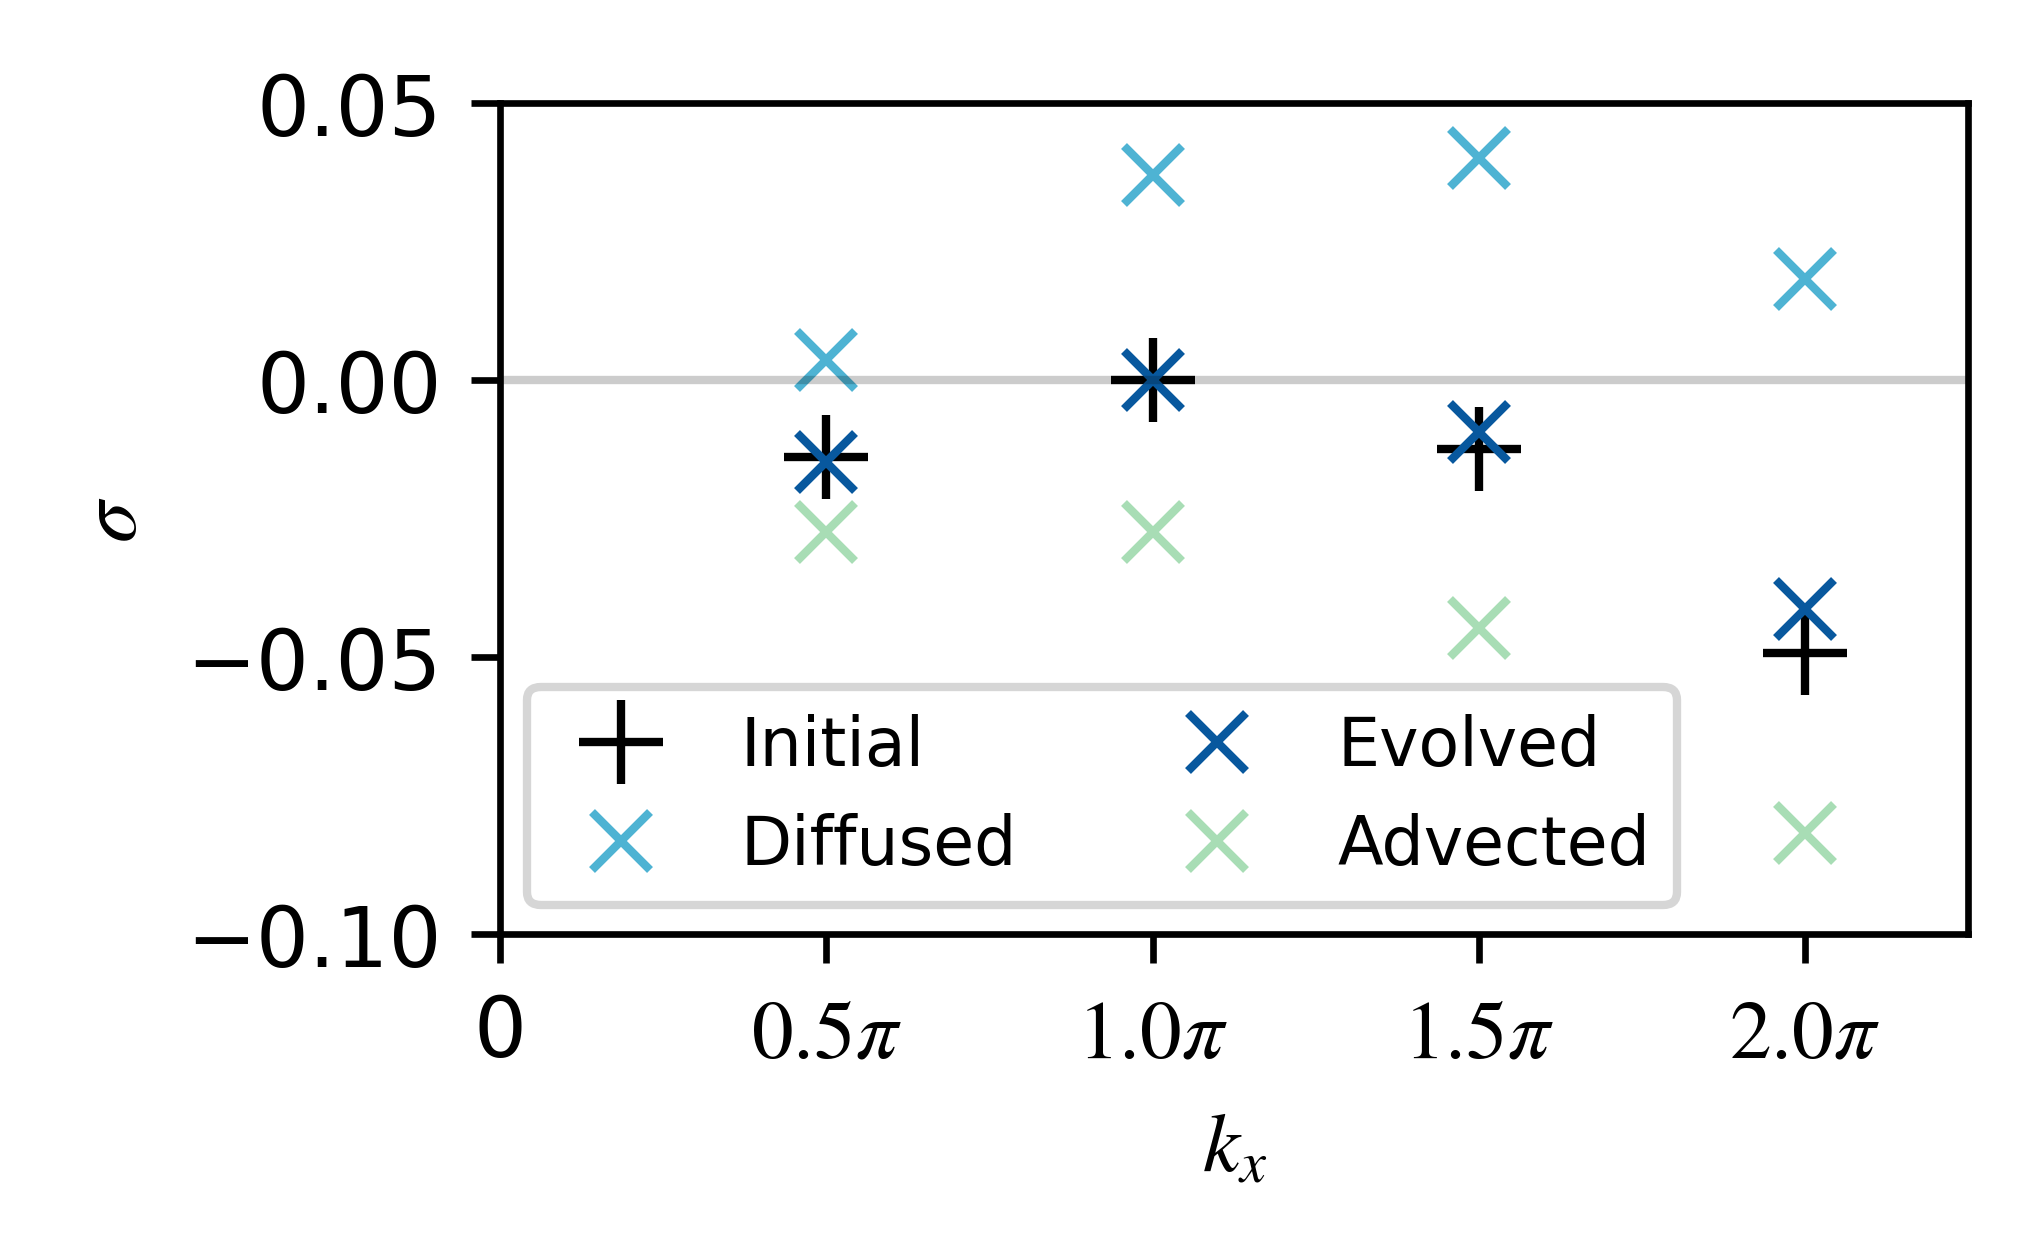
\includegraphics[width=3.4in]{EV_spectrum_ol.png}
    \caption{Eigenvalue spectra for $\Ra = 10^5$. The spectrum of an ``initial" marginally-stable mean temperature profile $\bar{T}(z, t_0)$ has a maximum eigenvalue of 0. 
    Given a small fixed timestep $\Delta t$, diffusion destabilizes the system, increasing its eigenvalues. 
    Advection tends to stabilize the system, decreasing its eigenvalues. 
    We find the eigenfunction amplitude $A^2$ such that the combination of diffusion and advection yields a new, ``evolved,'' marginally-stable mean temperature profile $\bar{T}(z, t_0 + \Delta t)$.}
    \label{fig:iteration_spectra} 
\end{figure}

An iteration is performed as follows.
Consider a marginally-stable temperature profile $\bar{T}(z, t_0)$.
By definition, its maximum eigenvalue is 0.
Diffusing $\bar{T}(z, t_0)$ tends to increase its eigenvalues.
Ignoring the diffusive term and evolving according to advection tends the stabilize the system.
The appropriate amplitude $A^2$ can then be approximated by
\begin{equation}
    A^2 \approx -\frac{\sigma_{\rm{diff}}}{\sigma_{\rm{adv}}} \label{EQ:amp_approx}
\end{equation}
where $\sigma_{\rm{diff}}$ and $\sigma_{\rm{adv}}$ refer to the diffused and advected eigenvalues of the initially marginal mode.
We illustrate these trends in Figure~\ref{fig:iteration_spectra}. 
$\bar{T}(z, t)$ is then evolved according to \eq{EQ:T0_IVP} and another eigenvalue solve is performed. 
Given a fixed timestep $\Delta t$, we assume the dominant eigenvalue can be described by a continuous function $\sigma_{\rm{max}} (A^2)$ which is locally differentiable. 
We use Newton's method to find an amplitude which satisfies our marginal stability tolerance criterion $|\sigma_{\rm{max}} (A^2)| < 10^{-9}$.
Marginally-stable modes do not osscillate in time, i.e. $\sigma = 0$ implies $\omega = 0$.
This agrees with the convectional notion of exchange of stabilities \cite{drazin_reid_2004}.
Crucially, we do not assume the $k_x$ of the marginally-stable is fixed.
In section \ref{sec:multiple_modes} we specify procedures for the treatment of multiple simultaneously marginal modes.

\subsection{Treatment of multiple marginally-stable modes} \label{sec:multiple_modes}
In most cases, we eventually encounter eigenvalue spectra with multiple simultaneously marginal modes.
If ignored, we are forced to reduce the timestep and allow the modes to alternate which is marginally stable.
Instead, we generalize the advective term in \eq{EQ:T0_IVP} to accommodate $N$ simultaneously marginal modes
\begin{equation}
    \langle w' T' \rangle_x = \sum_{n = 1}^{N} 4 A_n^2 \int \, \Re\left[ W_n \theta_n^* \right] \,dz
\end{equation}
where $W_n$ and $\theta_n$ are the eigenmodes associated with $k_x = \frac{n\pi}{2}$. 
There are now $N$ amplitudes to solve for and $N$ eigenvalues to keep marginally-stable. 
Given a small fixed time step $\Delta t$, let $\vec{A^2}$ be the amplitude vector and $\vec{\sigma}(\vec{A^2})$ be the dependent eigenvalues.
We expect a function $\vec{\sigma} \, : \, \mathbb{R}^N \to  \mathbb{R}^N$ to have isolated roots $\vec{A^2_m}$ (should they exist). 
The appropriate amplitude vector $\vec{A^2_m}$ can be approximated by a generalized form of \eq{EQ:amp_approx}:
\begin{equation}
    \vec{A^2_m} \approx -\Sigma_{\rm{adv}}^{-1} \vec{\sigma_{\rm{diff}}}.
    \label{EQ:AN_approx}
\end{equation}
Here $\vec{\sigma_{\rm{diff}}} = \vec{\sigma} (\vec{0})$ refers to the eigenvalues after a brief $\Delta t$ period of diffusion. 
$\Sigma_{\rm{adv}} \in \mathbb{R}^{N \times N}$ is the matrix of eigenvalues after $N$ $\Delta t$ periods of advection (one for each mode).
% The $k$th row of $J_0$ is then given by the gradient of the $k$th mode's eigenvalue $\nabla \sigma_k$.
In this way, an arbitrary element of $\sigma_{\rm{adv}}$ represents how a particular mode's eigenvalue responds to the advection of another mode. 
Solving \eq{EQ:AN_approx} gives a coarse estimate for $\vec{A^2_m}$. 
We refine our estimate by approximating the Jacobian matrix of $\vec{\sigma}(\vec{A^2})$ via first-order finite differences at the point of our coarse estimate.
This involves $N^2$ more individual EVP solves.
After its construction, the Jacobian is updated with each guess according to Broyden's method for root-finding in multi-dimensional functions \cite{Broyden}.
We find $\vec{\sigma}(\vec{A^2})$ does indeed have a unique root provided the time step is not too large and there are no numerical instabilities, as outlined in appendix \ref{sec:timestep}.
Presumably this is due to the dependence of $W(z)$ and $\theta(z)$ on $\bar{T}$.
Over the course of a large time step, $\bar{T}$ evolves according to \eq{EQ:T0_IVP} and the eigenfunctions might cease to provide a stabilizing influence.

Difficulty arises when transitioning between different numbers of marginal modes, particularly when stable modes become marginally-stable mid-iteration.
We facilitate these transitions by defining an adjustable candidate tolerance $\varepsilon_{\rm{cand}} \in [10^{-6}, 10^{-8}]$.
We rely on $A^2 > 0$ by asserting that a mode which meets the candidate tolerance can be included in an iteration provided that its respective amplitude is positive.
Should that be the case, the candidate mode is now marginally-stable and included in the subsequent iteration.
If however we converge on a negative amplitude, the candidate mode is discarded and the iteration is repeated. 
%In general we find that no other obvious course of action yields equilibria.

After several time steps, $\bar{T}$ tends to asymmetrize due to numerical noise. 
Though asymmetric pairs of solutions may exist, we further constrain $\bar{T}$ by imposing symmetry. 
This is accomplished at the start of each iteration by setting the coefficients of even Chebyshev polynomials to zero.

\section{Properties of Thermally Equilibrated States}\label{sec:properties}
We evolve $\bar{T}$ as described above until $|\partial_{t}\bar{T}| < 10^{-5}$.
In this marginally-stable thermal equilibrium, $\bar{T}$ does not evolve in time, and the perturbations also do not evolve in time, as they are marginally stable.
Thus, these configurations are exact solutions to the quasilinear equations (equations~\ref{EQ:T0_IVP}--\ref{EQ:linear3}).
They differ from the usual ECS in that ECS are fixed points of the full nonlinear problem \eqss{EQ:motion1}{EQ:motion3}. 
Such definitions are not mutually exclusive, but in general we can assume that MSTE and ECS are not steady with respect to their counterparts' equations.
We compute symmetric MSTE for $\Ra$ in the range $10^5 - 10^9$.

\begin{figure}
    \centering
    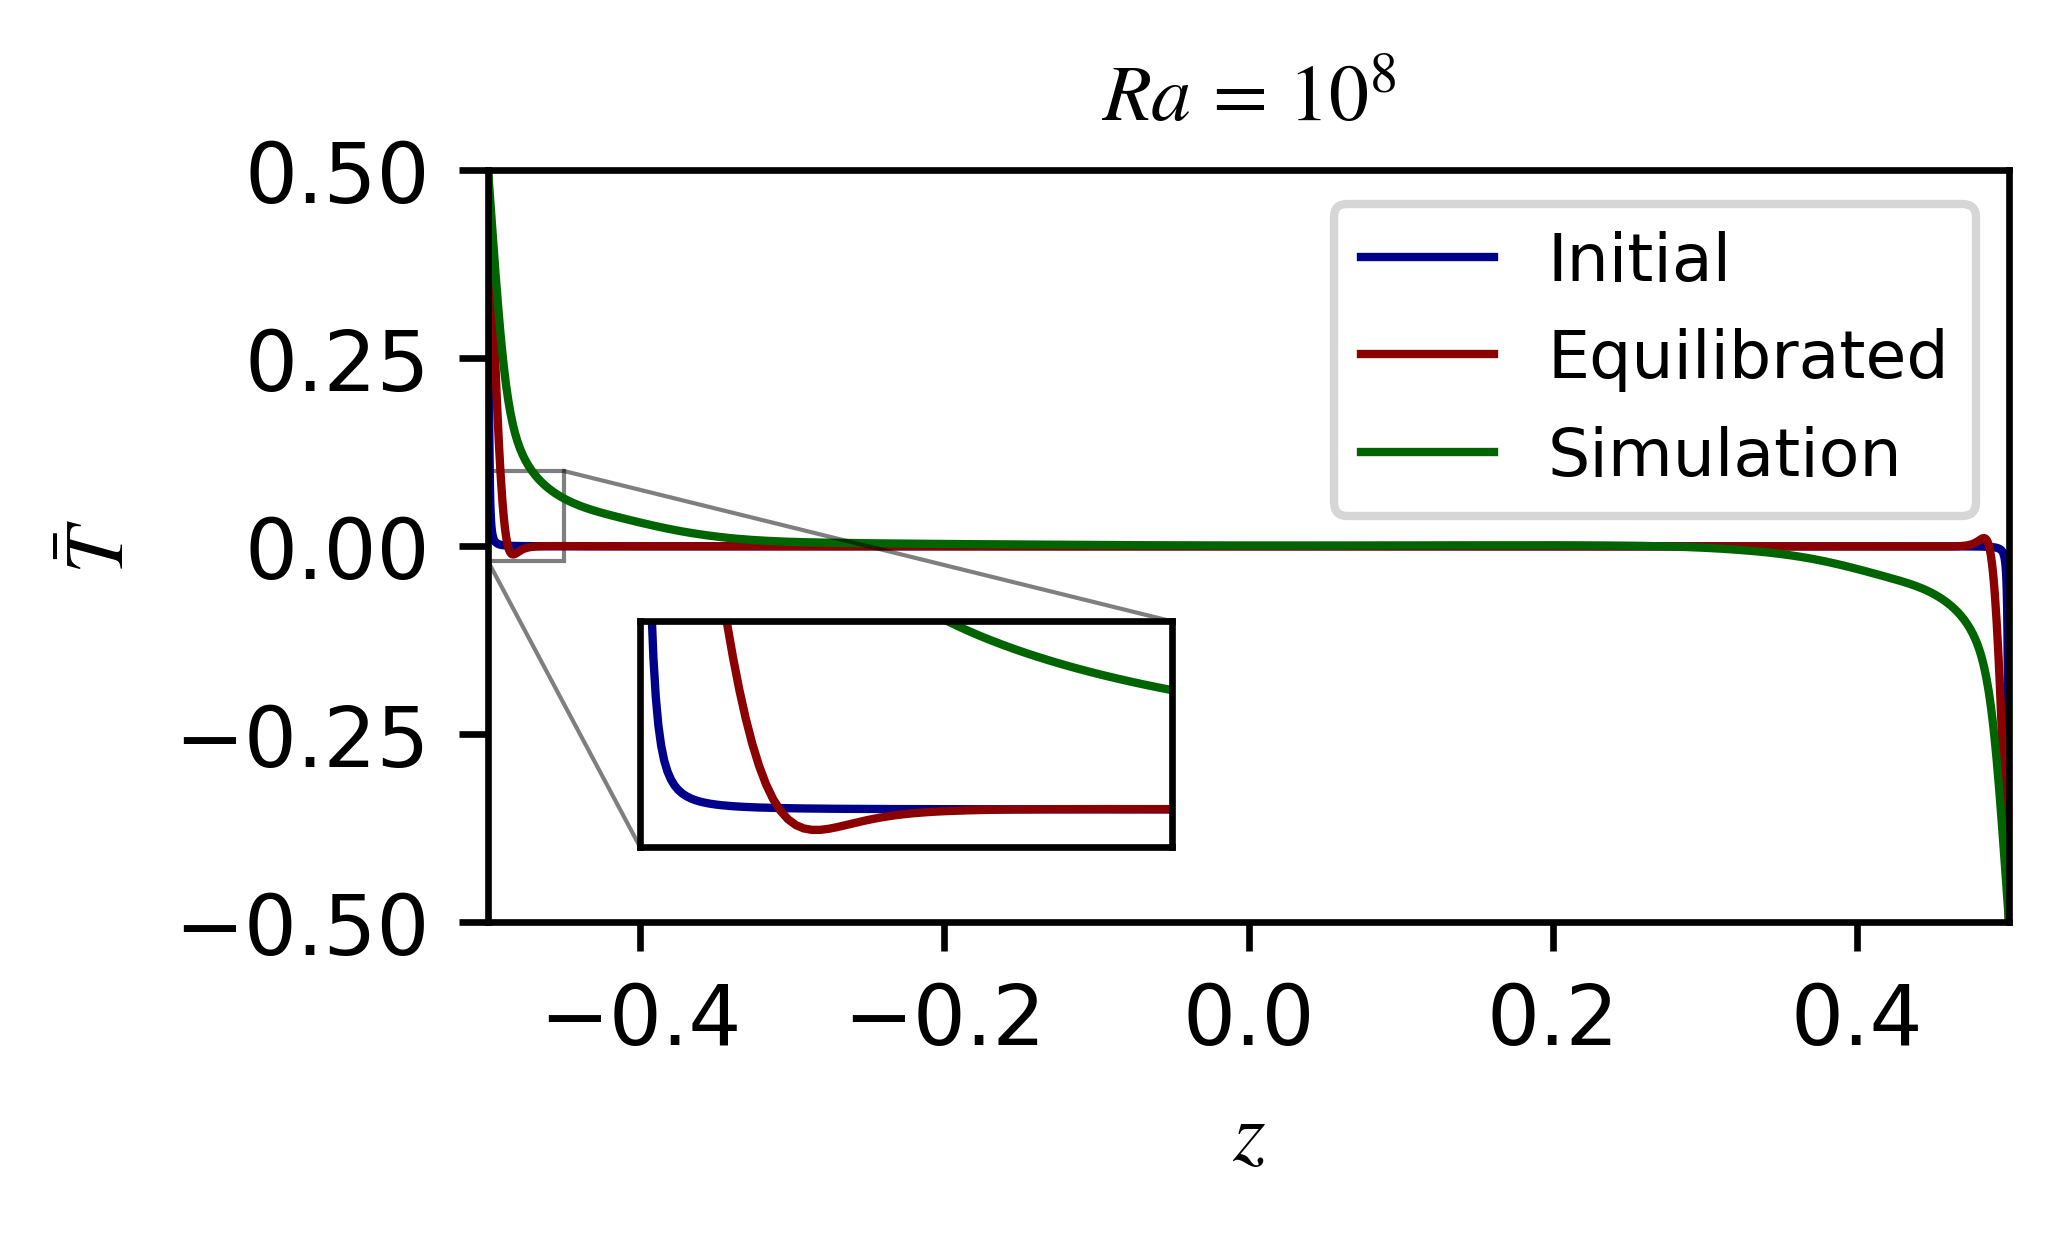
\includegraphics[width=3.4in]{T_profs_na.png}
    \caption{Mean temperature profiles $\bar{T}$ for $\Ra = 10^8$. 
    The initial profile is given by \eq{EQ:T0}. 
    We evolve this background temperature profile according to section~\ref{sec:evolution} until we reach a marginally-stable thermal equilibrium (MSTE).
    The DNS curve is obtained from a 2D nonlinear simulation of \eqss{EQ:motion1}{EQ:motion3} with \texttt{Dedalus}.
    DNS temperature data are horizontally- and time-averaged.
    The initial profile has the narrowest boundary layer, while the DNS profile has the widest boundary layer.
    The MSTE profile exhibits prominent dips, nested alongside the boundary regions. }
%    The source of this feature is not well understood, but similar temperature gradient reversal regions were found by \cite{chini_cells} along the midlines of 2D convective cellular solutions at $\Ra \sim 10^6$.}
    \label{fig:T0_profiles}
\end{figure}

Figure \ref{fig:T0_profiles} gives temperature profiles for $\Ra = 10^8$ where the initial profile, whose construction is outlined in appendix~\ref{sec:initial_profile}, is employed at iteration 0. 
Direct numerical simulations (DNS) are performed by solving \eqss{EQ:motion1}{EQ:motion3} with \texttt{Dedalus}, followed by horizontal- and time- averaging. 
The DNS curve is more diffuse than the MSTE curve, which in turn, is more diffuse than the initial curve. 
Performing an eigenvalue solve by setting $\bar{T}$ equal to the DNS profile yields unstable eigenvalues. 
This suggests that MSTE might maximize boundary layer thickness, subject to the marginal stability constraint.

\begin{figure*}
    \centering
    \begin{tabular}{@{}c@{}}
        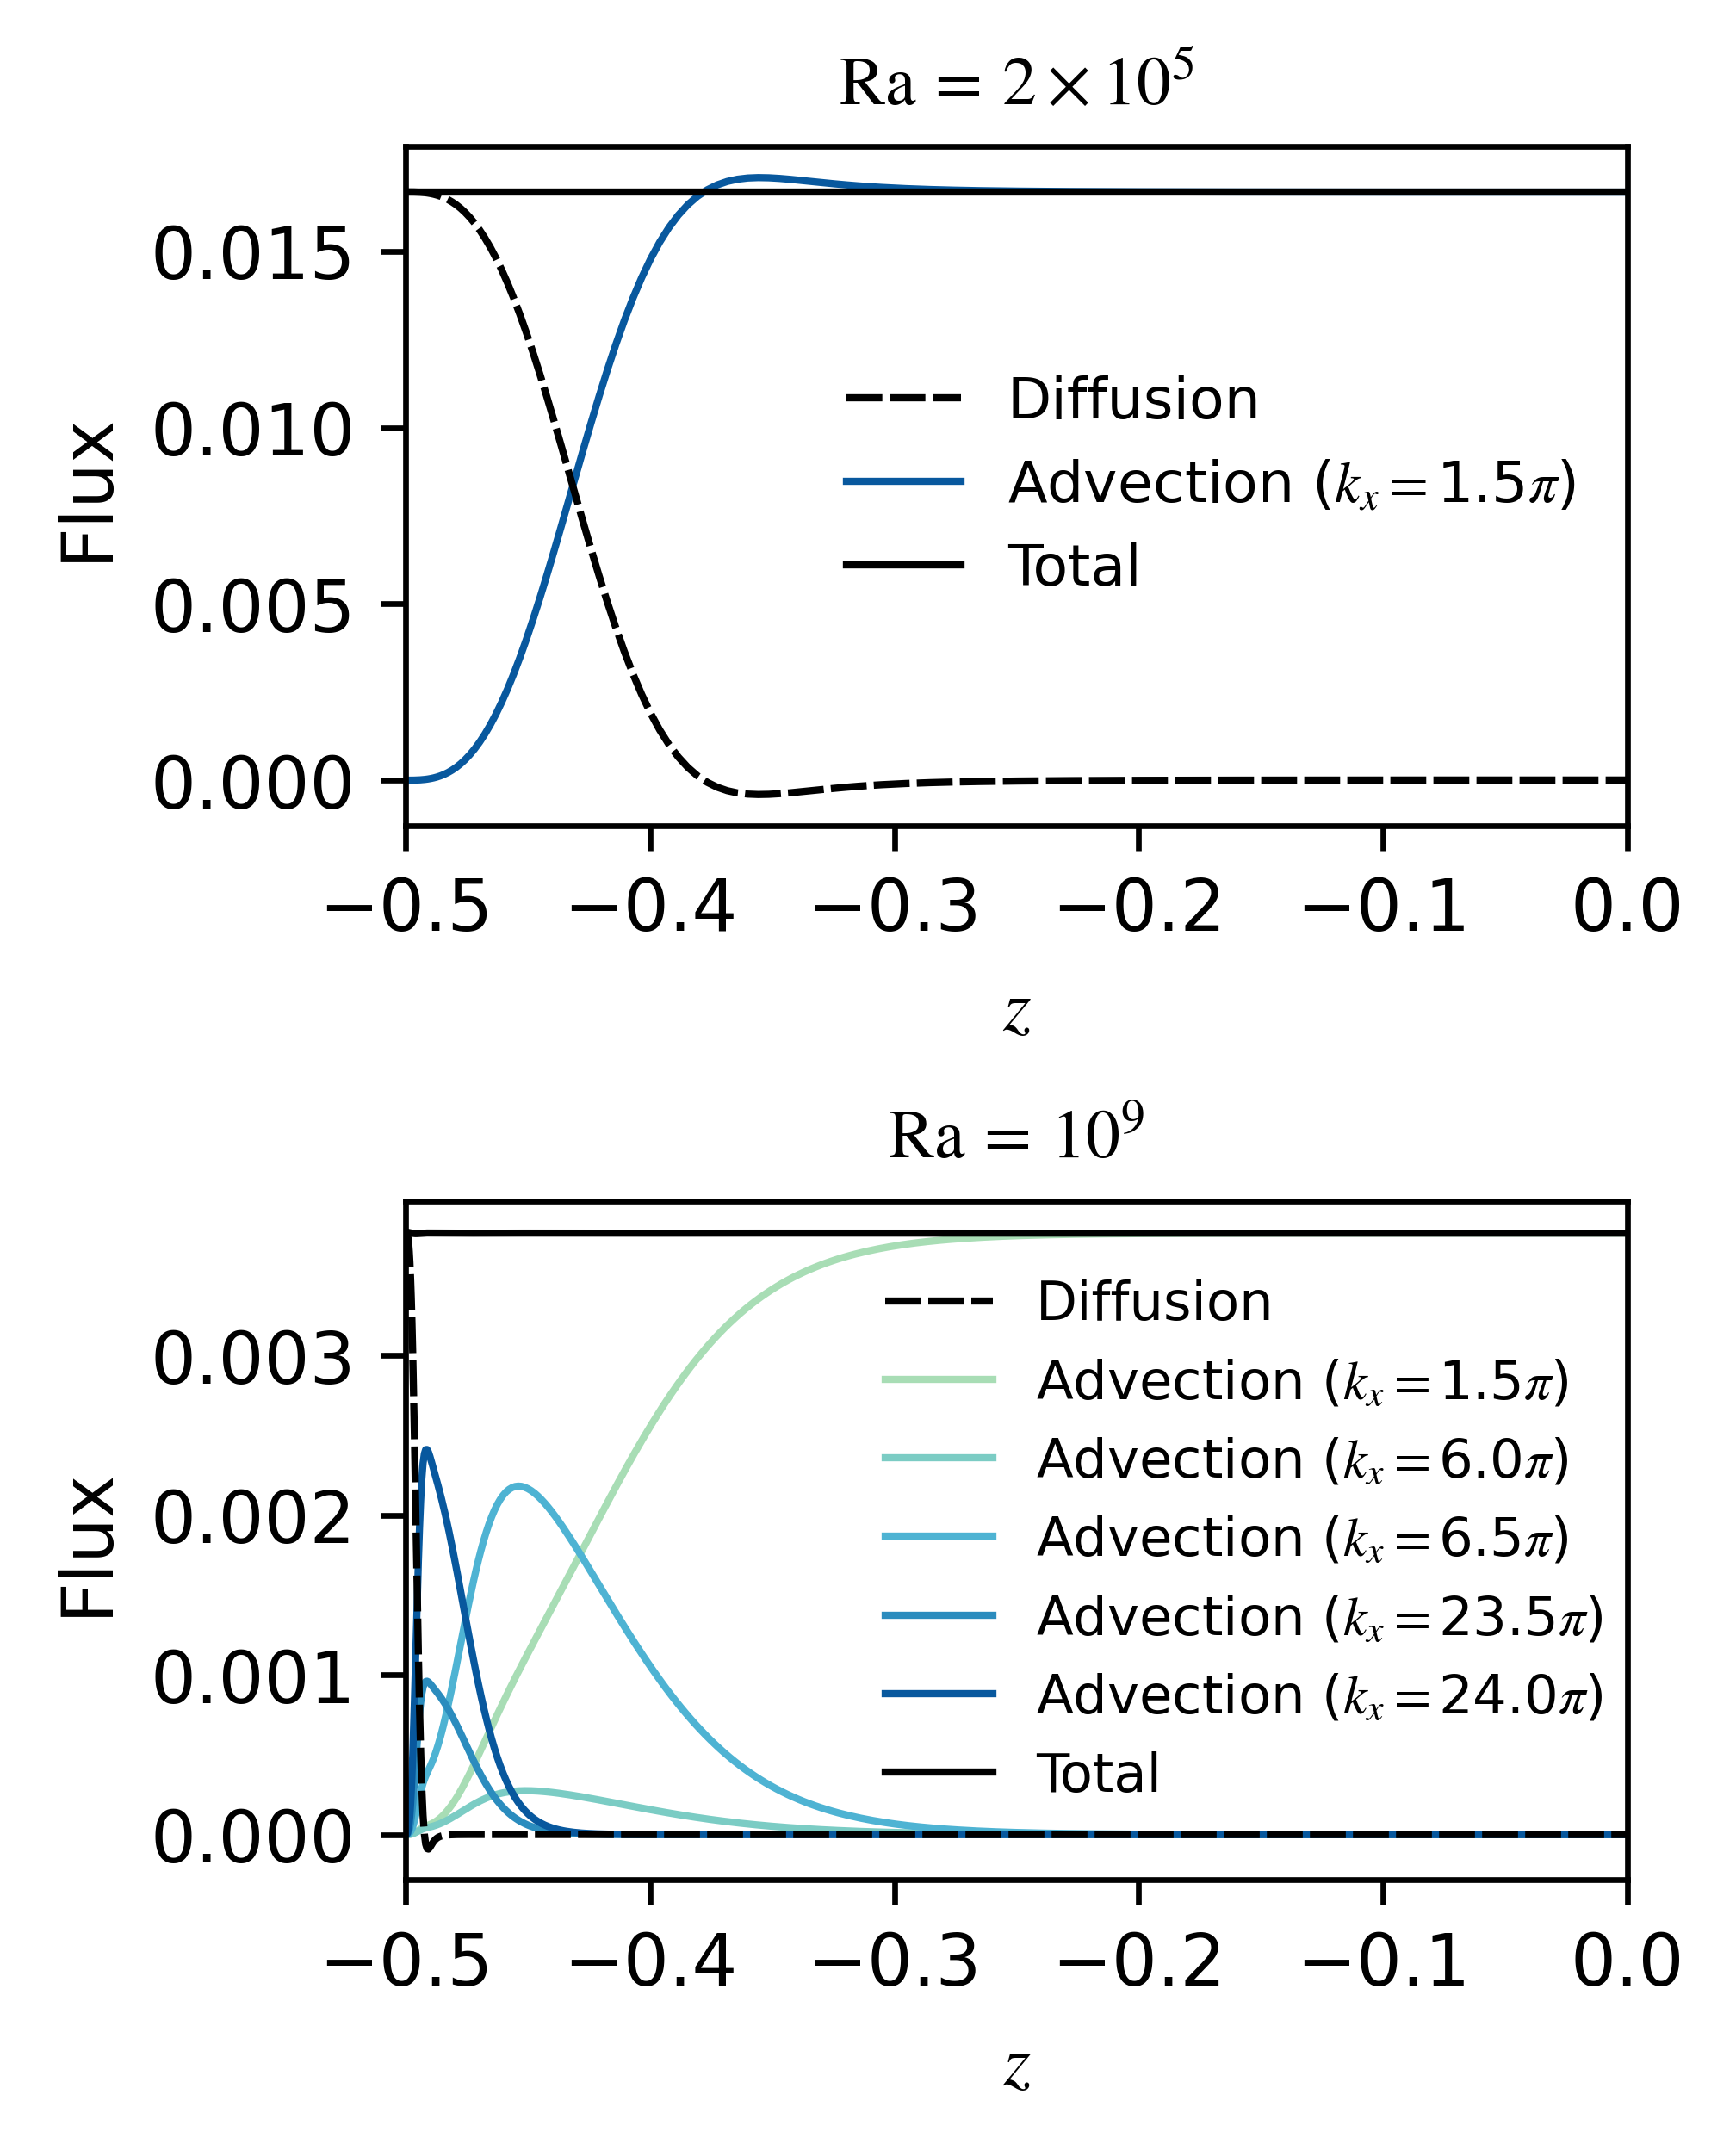
\includegraphics[width=3.4in]{flux_sup_n.png}
    \end{tabular}
    \begin{tabular}{@{}c@{}}
        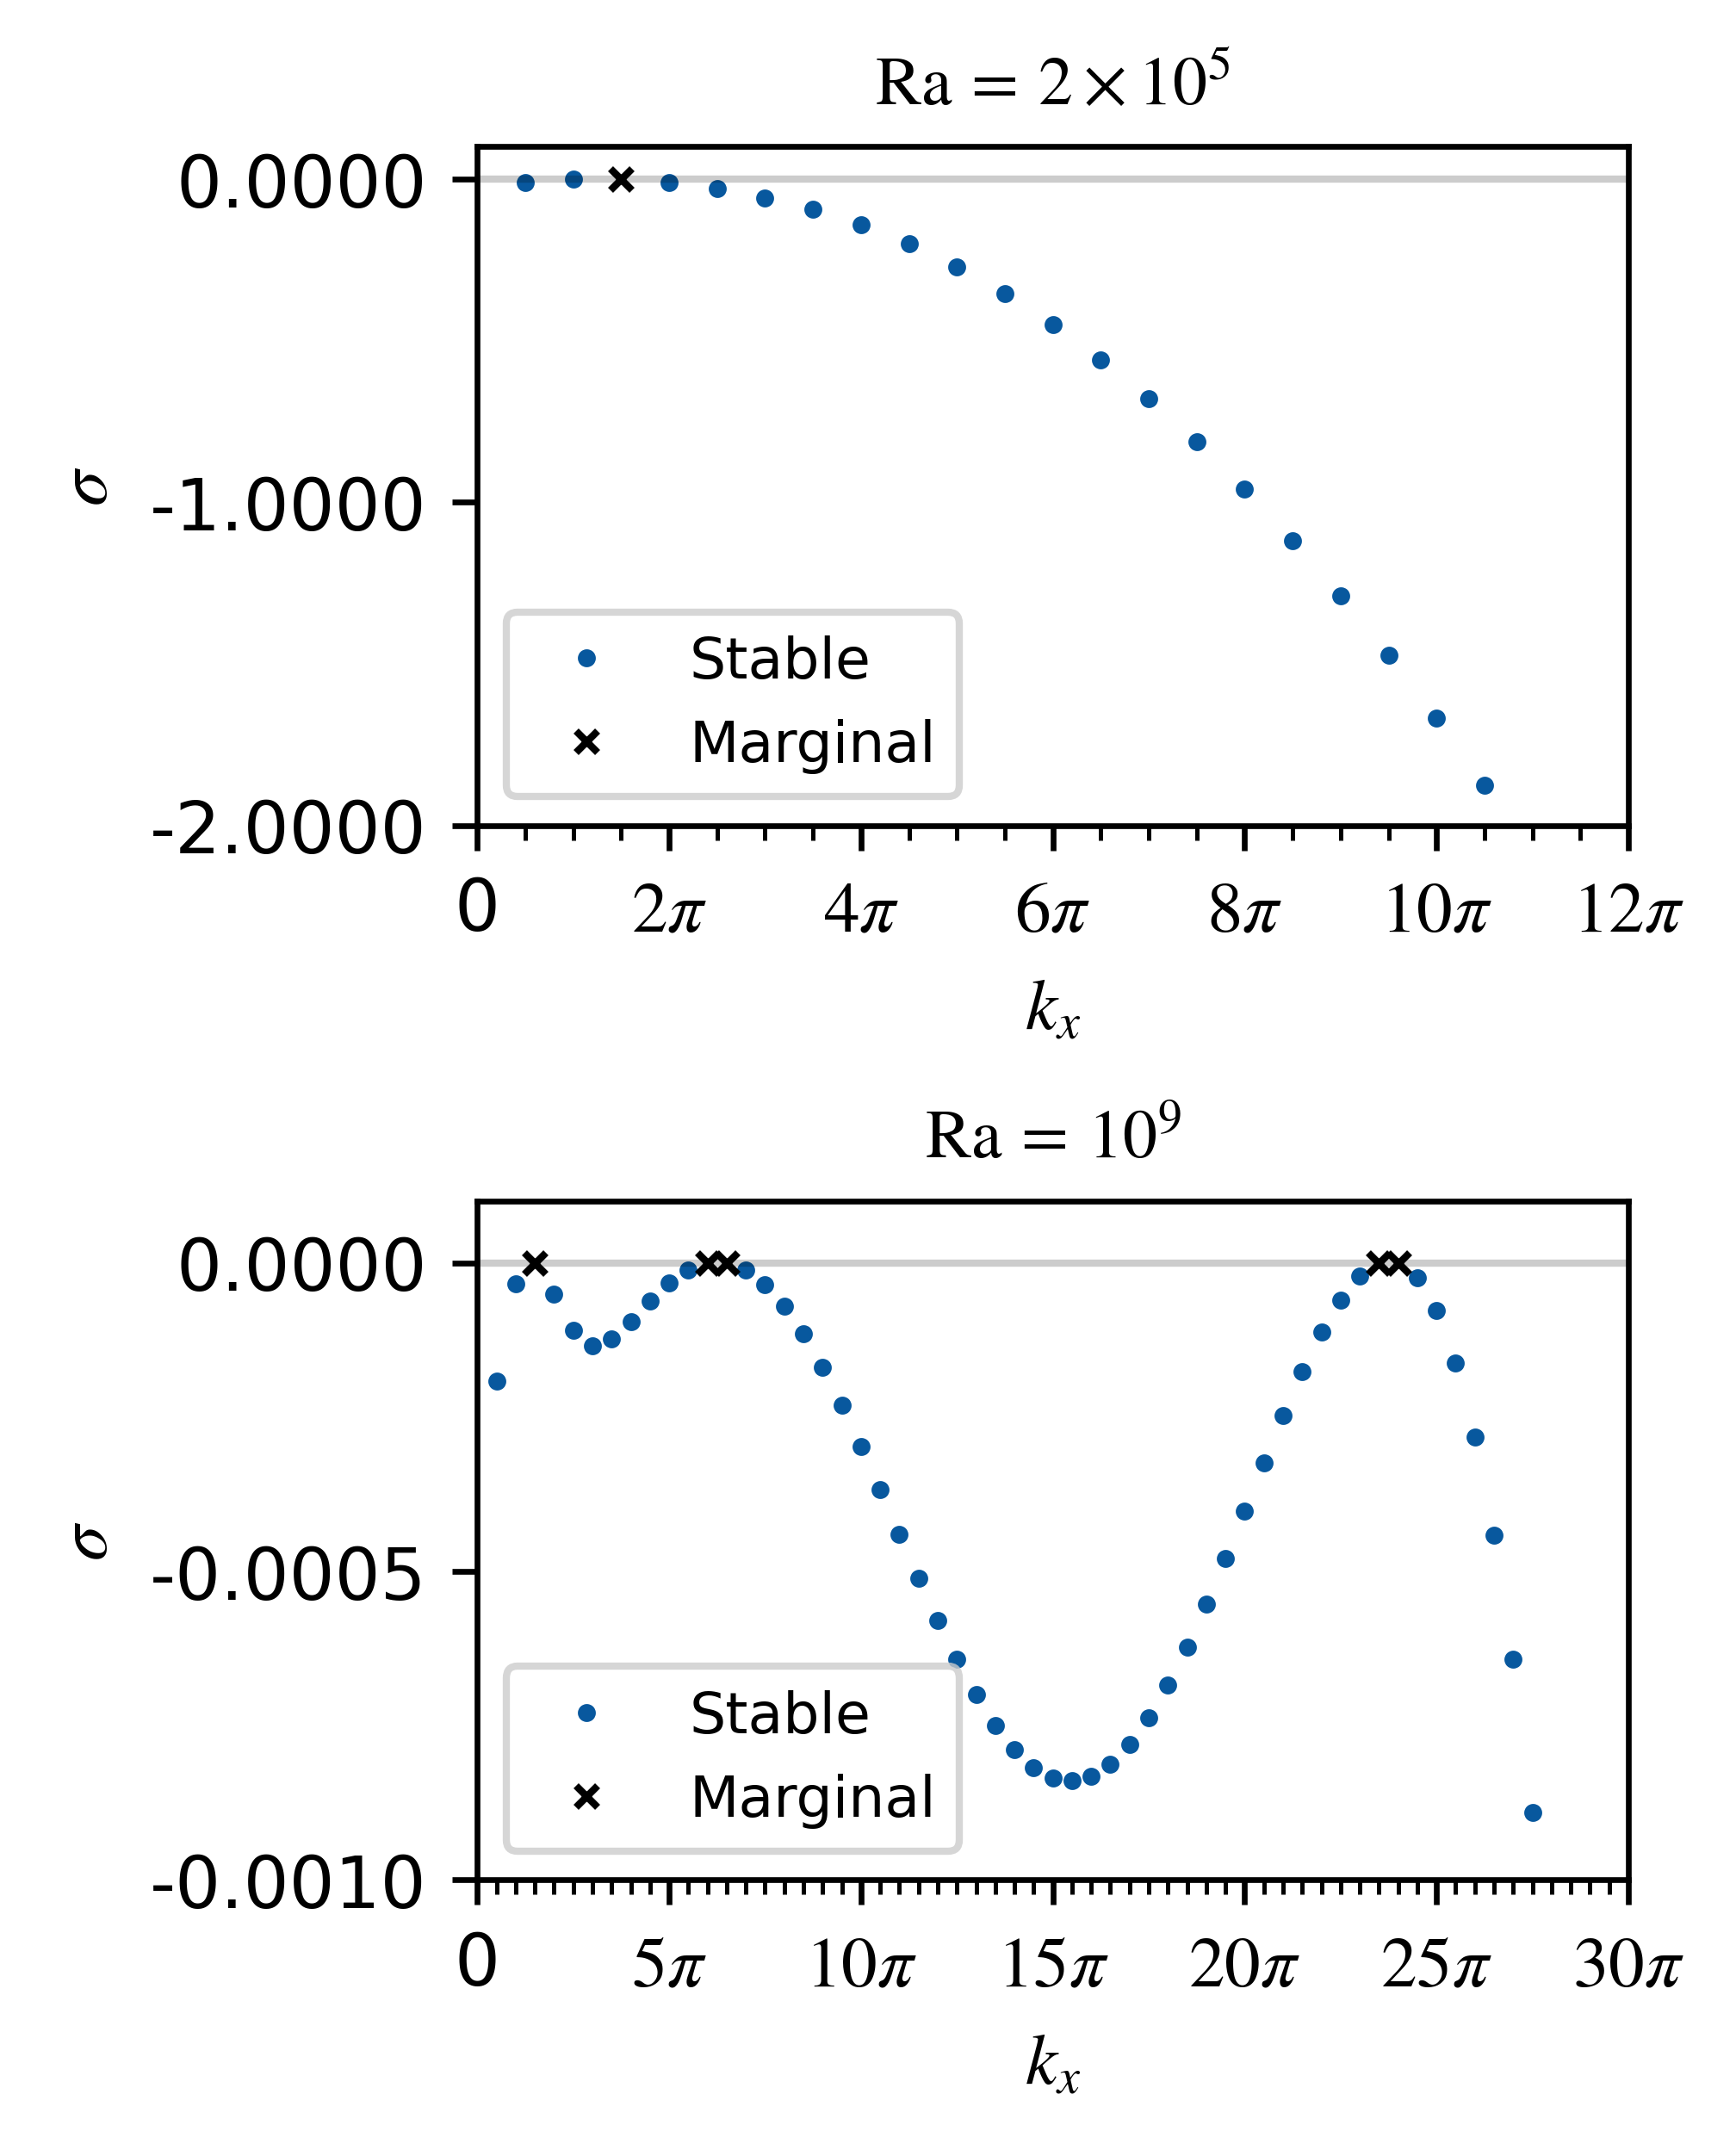
\includegraphics[width=3.4in]{EV_spectra_2ra.png}
    \end{tabular}
    \caption{Heat fluxes (left) and eigenvalue spectra (right) of equilibrated states $\Ra = 2 \times 10^5$ (top) and $\Ra = 10^9$ (bottom). 
    The heat flux profiles are symmetric about $z=0$, so we only plot for $z<0$.
    Advection profiles belong to marginally-stable modes. 
    For low $\Ra$, a single mode with $k_x = 1.5\pi$ is sufficient to oppose boundary layer diffusion and facilitate heat flux throughout the bulk of the domain. 
    For large $\Ra$, high-wavenumber modes contribute pronounced small-scale advection profiles which tightly hug the thin boundary layers. 
    A combination of of progressively wider advection profiles is necessary to transition to the $k_x = 1.5\pi$ mode.}
    \label{fig:flux}
\end{figure*}

The most resilient and unexpected feature of MSTE temperature profiles are the pronounced dips adjacent to the boundary layers. 
These dips appear in every solution, regardless of $\Ra$. 
Physically, they correspond to thin layers in which the mean temperature gradient reverses, contradicting an important hypothesis of \cite{Malkus_1954,Howard_1966}. 
This counter-diffusion, which opposes overall heat transfer, is overcome by the coinciding advective flux, shown in Figure \ref{fig:flux}. 
We do not understand the source of these dips, but similar temperature gradient reversals were reported by \cite{chini_cells} along the midlines of 2D convective cellular solutions at $\Ra \sim 10^6$.
In that case, the reversals were due to nonlinear advection, which is not present in our quasilinear model. 

Equilibrated states exhibit distinct behaviors for large and small $\Ra$. 
This contrast is illustrated in Figure \ref{fig:flux}, where we give heat flux profiles and eigenvalue spectra for two cases: $\Ra = 2 \times 10^5$ and $\Ra = 10^9$. 
For $\Ra = 2 \times 10^5$, there is a single marginal mode at $k_x = 1.5\pi$ whose advective flux occupies the bulk of the domain. 
These states have wide boundary layers which gradually subside as advection becomes the dominant flux component. 
Such transitional regions do not appear for $\Ra = 10^9$.
In this case the shift from diffusion to advection is sharp.
At $\Ra=10^9$ we find five marginally-stable modes are necessary to reach a MSTE.
Thin advection profiles, belonging to high-wavenumber modes with $k_x=23.5\pi, \, 24\pi$, hug the boundary layer. 
Closer to the bulk of the domain, we see wider advection profiles corresponding to modes in a second group of marginal modes $k_x = 6\pi, \, 6.5\pi$.
The $k_x = 1.5\pi$ mode forms the large-scale convective cell structures observed in DNS, again occupying the bulk of the domain.
The pairs of modes $k_x = 6\pi, \, 6.5\pi$ and $k_x=23.5\pi, \, 24\pi$ are each associated with a single maximum in our plots of growth rate $\sigma$ as a function of $k_x$ (lower right panel of Figure~\ref{fig:flux}).
If we allowed wavenumbers to vary continuously, there would be an unstable mode between these pairs of wavenumbers.
However, since we have fixed the horizontal size of our domain, we are left with pairs of discrete margin modes.

\begin{figure}
    \centering
    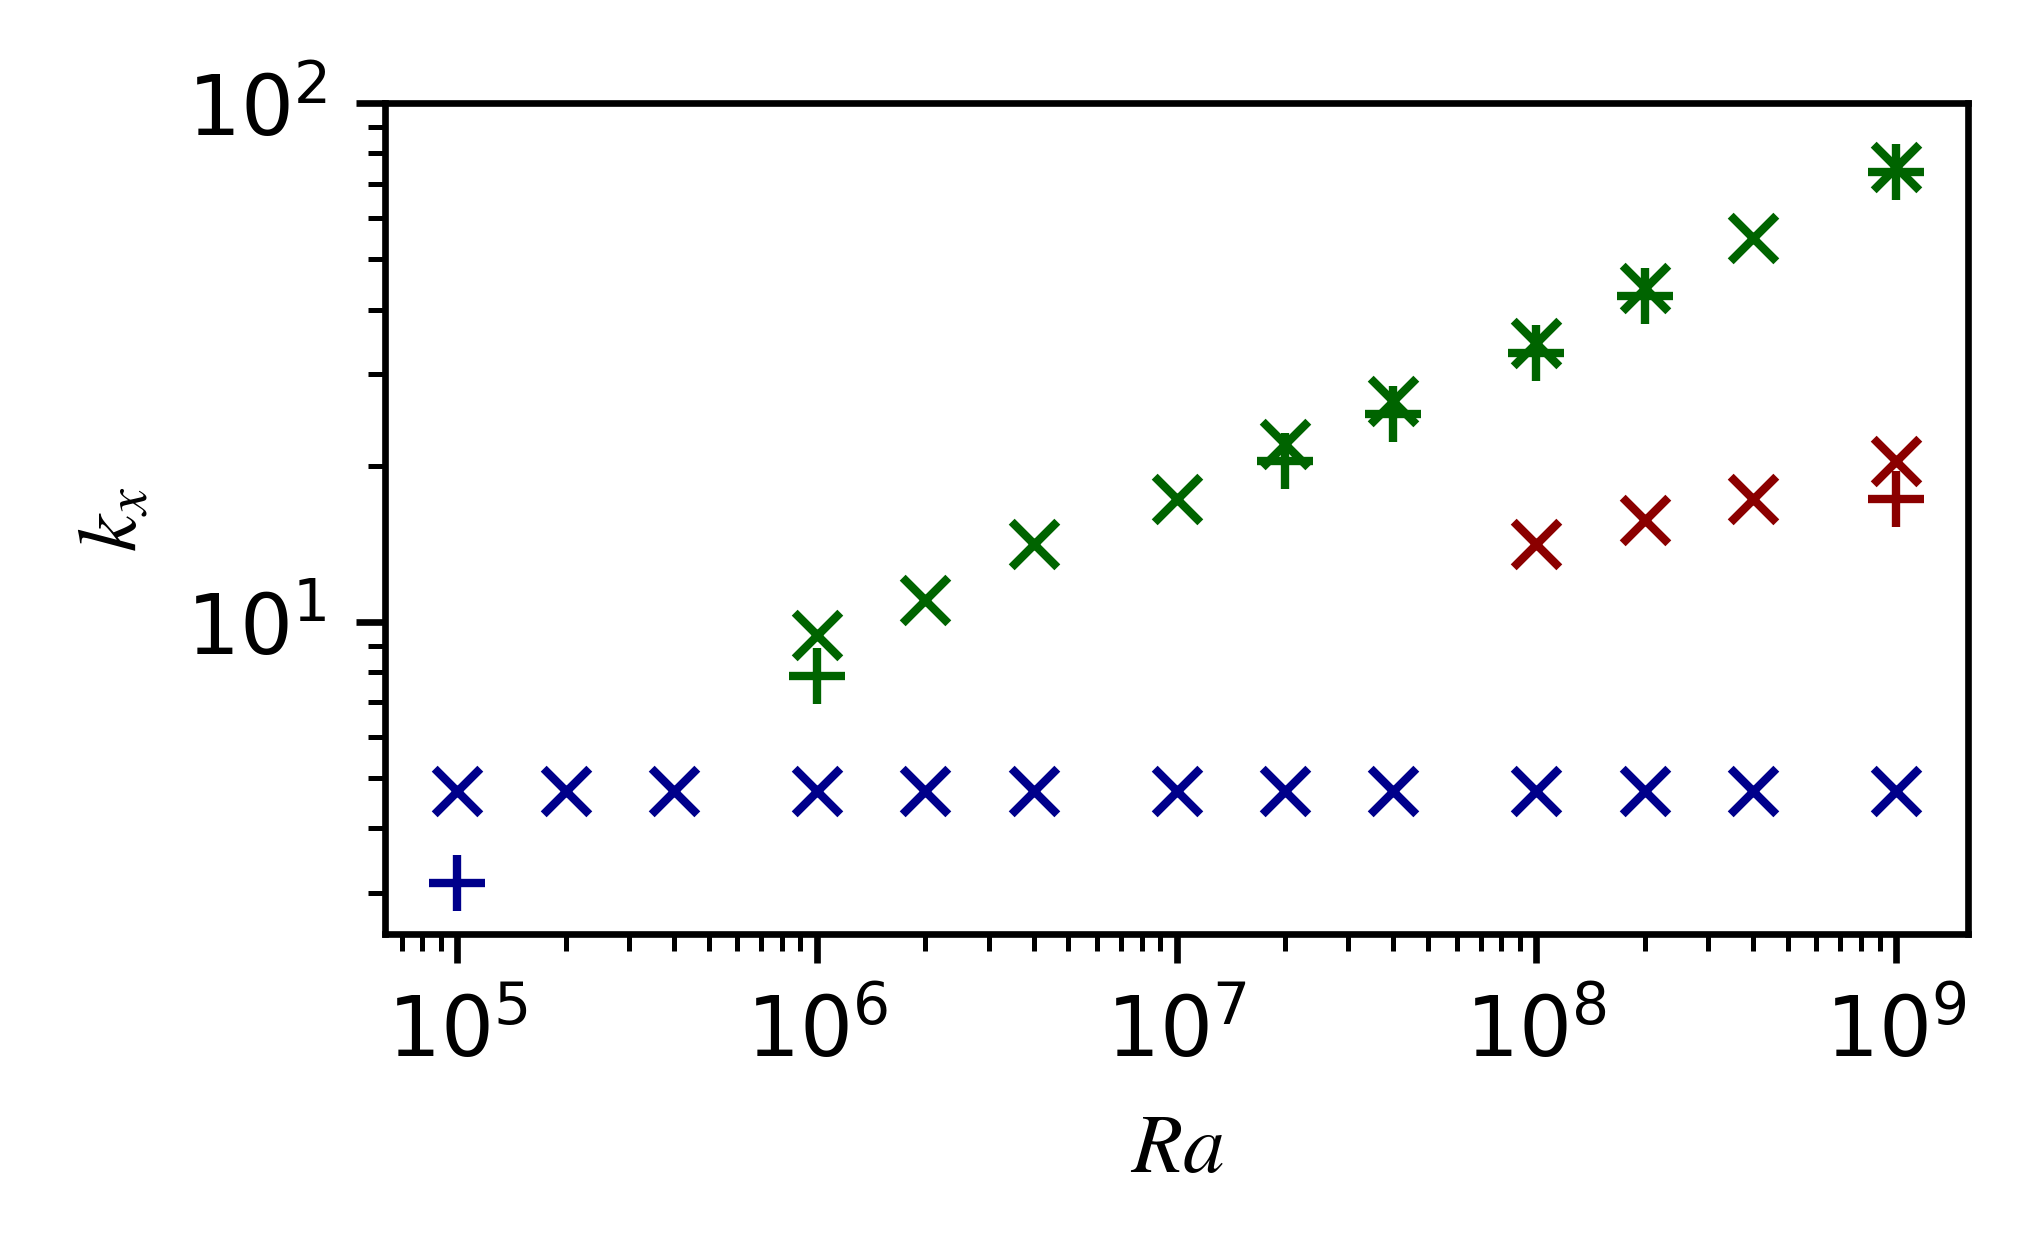
\includegraphics[width=3.4in]{kx_m_ra1.png}
    \caption{Wavenumbers of marginally-stable modes in thermally equilibrated states. 
    Marginal modes often appear in adjacent pairs, which we denote with a common color. 
    For example, the spectrum corresponding to $\Ra = 10^5$ has adjacent marginal wavenumbers $k_x = \pi, \, 1.5\pi$. 
    The $\Ra = 10^9$ spectrum, shown in lower right corner of Figure \ref{fig:flux}, has three groups of maxima, with a single marginal mode in the first group ($k_x = 1.5\pi$), two adjacent marginal modes in the second group ($k_x = 6\pi, \, 6.5\pi$), and two adjacent marginal modes in the third group ($k_x = 23.5\pi, \, 24\pi$). 
    The largest wavenumbers of the green branch obey a power-law relationship with $\Ra$}
    \label{fig:kx_marginals}
\end{figure}

MSTE for large $\Ra$ tend to have a diverse combination of marginal modes.
In every case, the $k_x = 1.5\pi$ mode is included. 
In Figure \ref{fig:kx_marginals} we give the wavenumbers $k_x$ of marginal modes. 
Sometimes we find two marginally-stable modes with wavenumbers separated by $\pi/2$.
Like $k_x = 6\pi, \, 6.5\pi$ and $k_x=23.5\pi, \, 24\pi$ for the $\Ra=10^9$ MSTE, these are due to the discretization of wavenumbers from our domain of width 4.
We think of the pairs of modes as acting together as part of a single maximum of the growth rate as a function of the wavenumber.
When wavenumbers are adjacent, we plot them in the same color and denote the larger mode with an x and the smaller with a +.
For $\Ra \geq 10^6$, a second branch of marginal modes is shown in light green. 
For large $\Ra$, the advective fluxes of this maximum branch opposes the strong diffusion of the thin MSTE boundary layers. 
At $\Ra \geq 10^8$, a third branch appears (shown in light blue), splitting the widening gap between the other two. 
This development is associated with moderately wide advection profiles, filling a niche in the total flux by uniting the thin profiles of the maximum branch with those of the bulk-domain-oriented minimum branch.

\begin{figure}
    \centering
    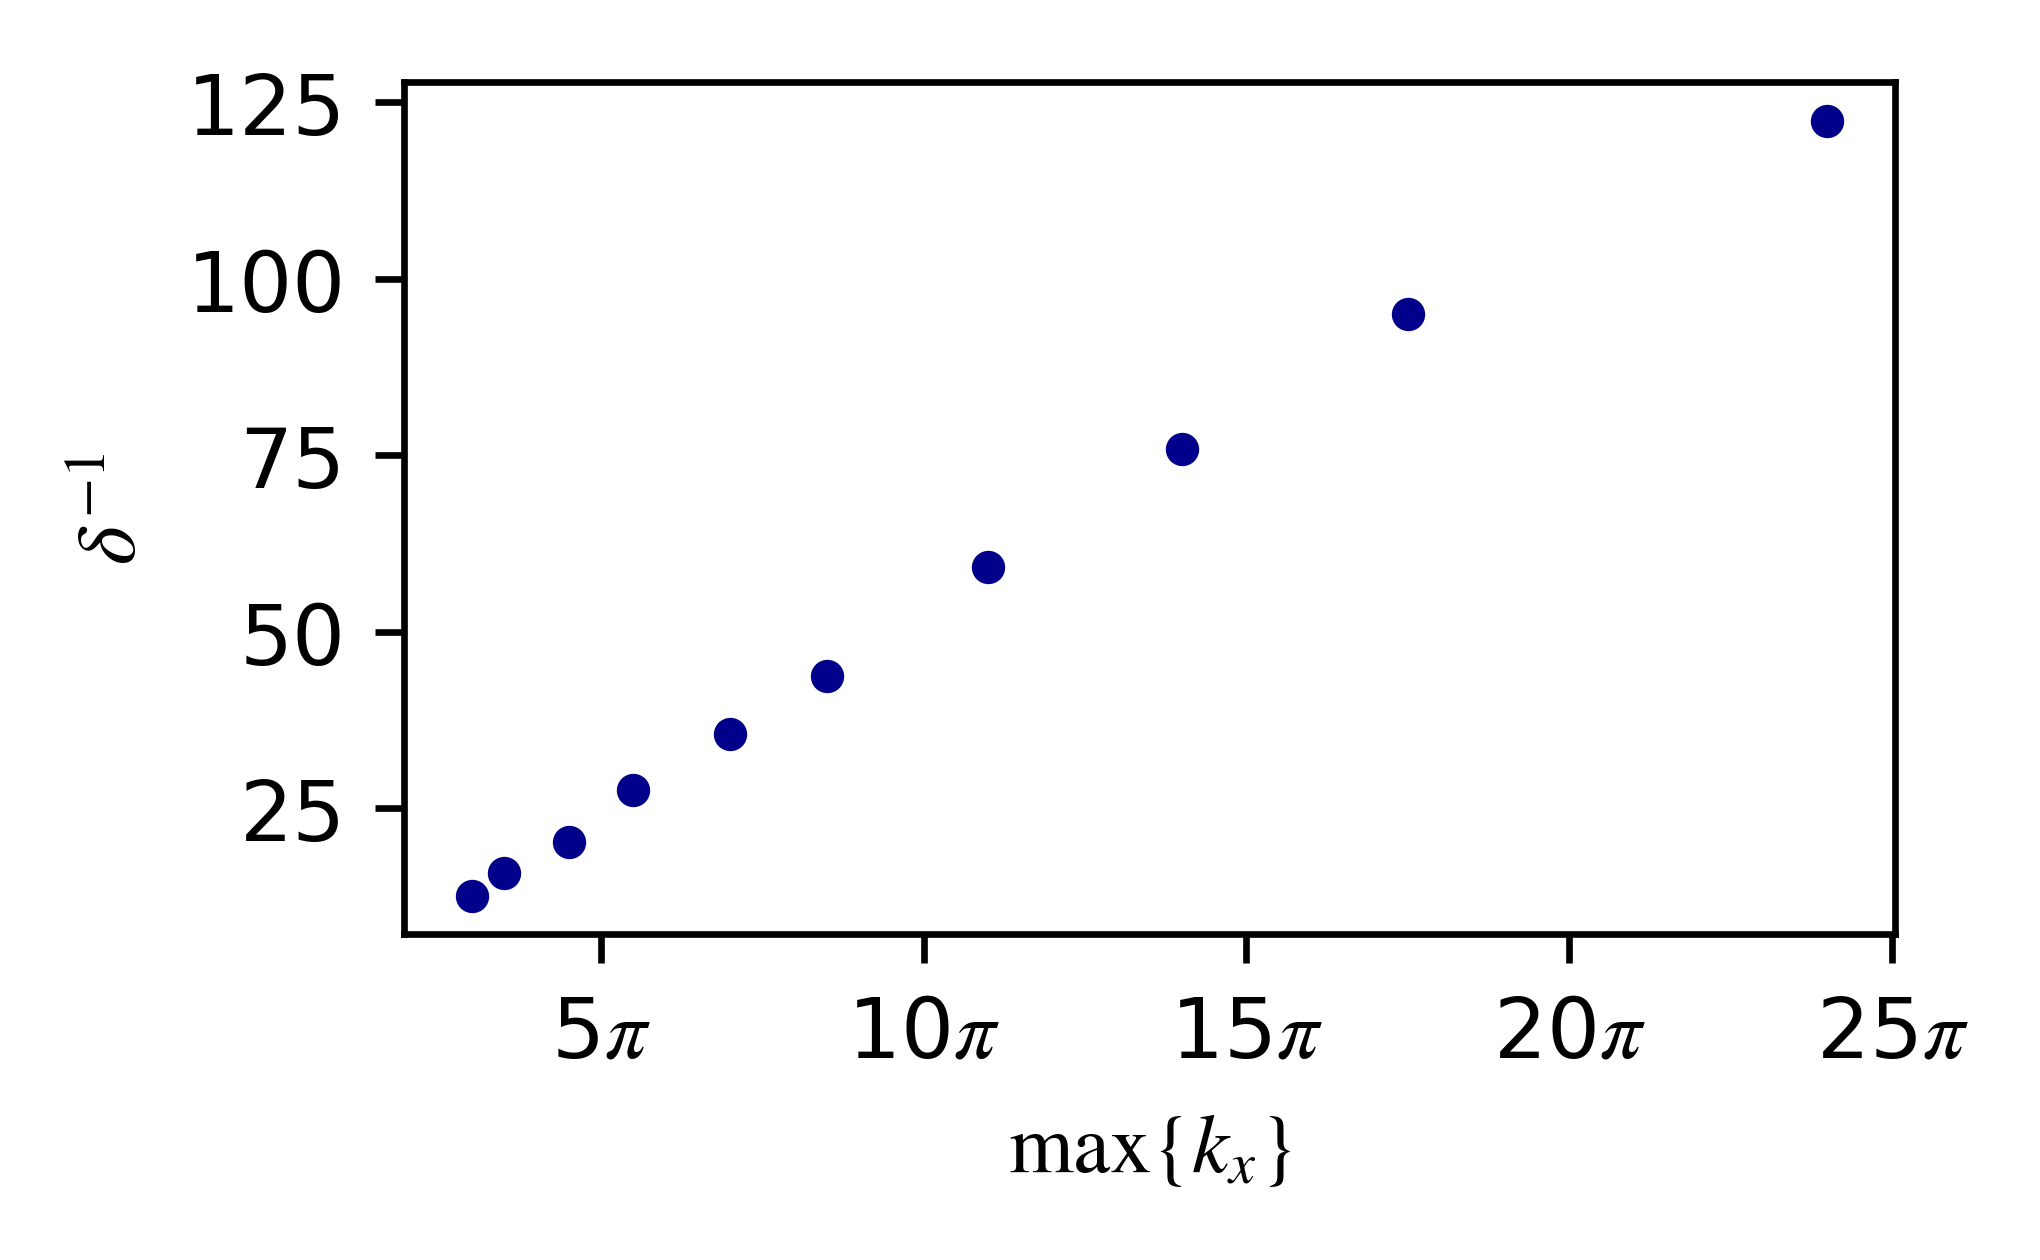
\includegraphics[width=3.4in]{del_kx_inv.png}
    \caption{For $\Ra \geq 10^6$, the maximum marginally-stable wavenumber (corresponding to the green x markers in Figure \ref{fig:kx_marginals}) are inversely related to the boundary layer height $\delta$. 
    $(\max \{ k_x \})^{-1}$ gives a minimum $x$ length scale for the perturbations, and consequently, the advection. 
    For large $\Ra$, the boundary layers admit small scale features, requiring more vertical basis functions (higher resolution).
    The boundary layer width gives an estimate of the minimum vertical lengthscale in the problem.
    This suggests that the minimum horizontal and vertical lengthscales are proportional to each other over a wide range of $\Ra$.}
    \label{fig:del_inv}
\end{figure}

The largest marginal wavenumber $\max \{ k_x \}$ (represented by the light green branch in Figure \ref{fig:kx_marginals}) serves as an inverse minimum length-scale in the $x$ direction.
The finest vertical structures in $\bar{T}(z)$ appear near the boundaries, requiring more basis functions (resolution) at large $\Ra$.
Naturally, this provides a complementary minimum length-scale for $z$.
We define the boundary layer width $\delta$ as the distance from the boundary where $\partial_z T$ equals zero, i.e.,
\begin{align}\label{eqn:delta}
\left.\frac{\partial \bar{T}}{\partial z}\right|_{z=-\frac{1}{2}+\delta} = 0.
\end{align}
This height corresponds to the local extrema of the MSTE temperature profile, e.g., in Figure \ref{fig:T0_profiles}.
In Figure \ref{fig:del_inv}, we show $\max \{ k_x\}$ is proportional to $\delta$ over our range of $\Ra$.
Least-squares regression gives $\delta^{-1} = 1.71 \max \{ k_x \} - 2.13$.
We can assume from this length scale agreement that the mean-squared $x$ and $z$ components of the temperature and velocity gradients are proportional
\begin{align}
    \Big\langle \frac{\partial T}{\partial x} \cdot \frac{\partial T}{\partial x} \Big\rangle_{\mathcal{D}} &\propto \Big\langle \frac{\partial T}{\partial z} \cdot \frac{\partial T}{\partial z} \Big\rangle_{\mathcal{D}} \nonumber   \\
    \Big\langle \frac{\partial \vec{u}}{\partial x} \cdot \frac{\partial \vec{u}}{\partial x} \Big\rangle_{\mathcal{D}} &\propto \Big\langle \frac{\partial \vec{u}}{\partial z} \cdot \frac{\partial \vec{u}}{\partial z} \Big\rangle_{\mathcal{D}}.
\end{align}
This is consistent with the mean squared gradient assumptions of \cite{Malkus_1954}.
%The quasilinear model cannot describe arbitrarily small scale structures. This is a consequence of us collapsing the problem into a single dimension via mode-discretization.

\begin{figure}
    \centering
    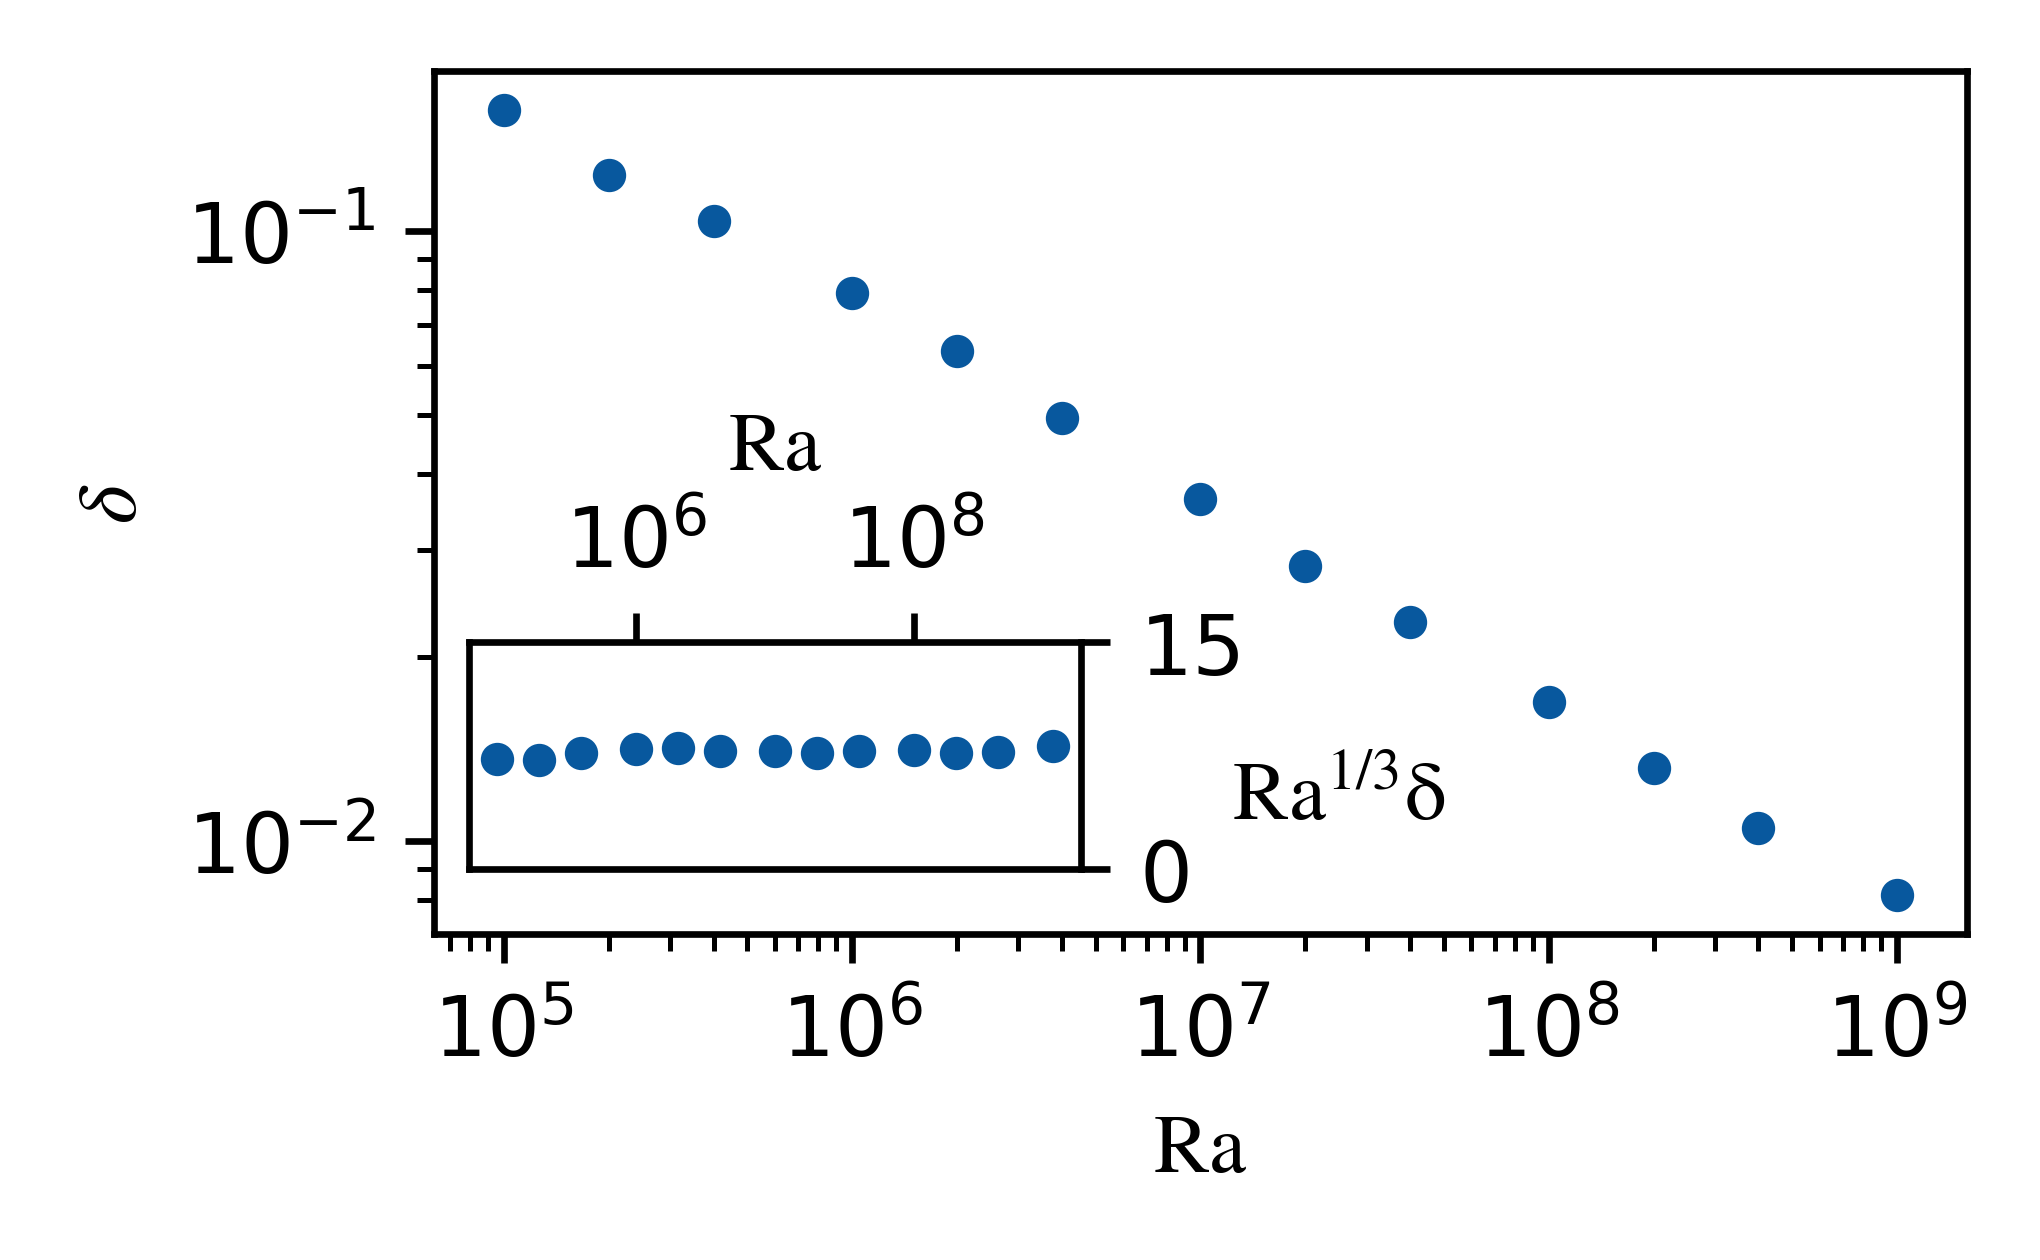
\includegraphics[width=3.4in]{del_ra.PNG}
    \caption{Boundary layer height $\delta$ of MSTE. 
    We define the boundary layer height based off the location where $\frac{\partial \bar{T}}{\partial z} = 0$ (see equation~\ref{eqn:delta}). 
    Plotting on a log-log scale, we find that $\delta$ and $\Ra$ obey a power-law relationship. We also demonstrate that $\Ra^{1/3}\delta$ is approximately constant with respect to $\Ra$ which is consistent with \cite{Malkus_1954}}
    \label{fig:bl_ra}
\end{figure}

We find the MSTE can be characterized by their boundary layer height.
In Figure \ref{fig:bl_ra}, we illustrate the scaling behavior of the boundary layer height $\delta = \Ra^{-1/3}$. 
This is consistent with Malkus' classical marginal-stability theory, a scaling argument which perceives the boundary regions as subdomains which are themselves marginally-stable \cite{Malkus_1954}.

\begin{figure*}
    \centering
    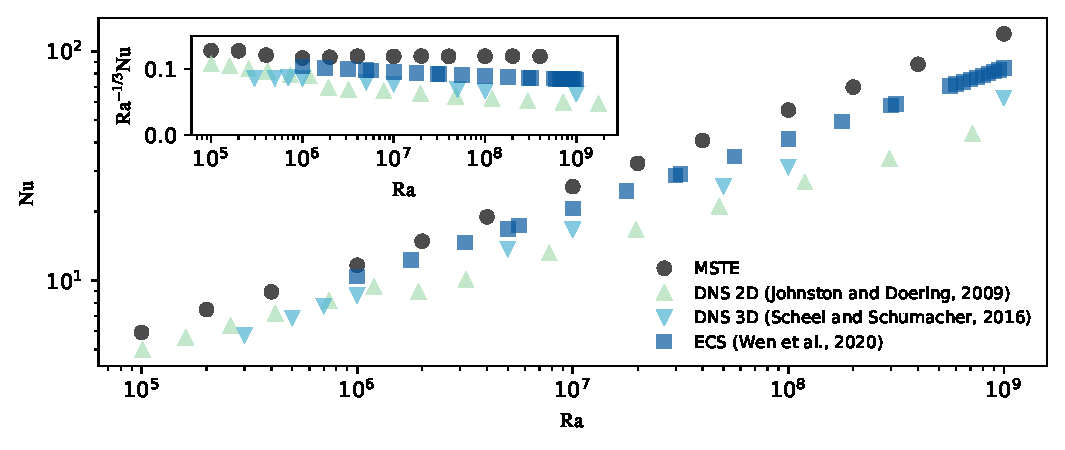
\includegraphics[width=7.1in]{nu_ra.PNG}
    \caption{Nusselt numbers are shown for MSTE, aspect-ratio-optimized ``steady rolls'' ECS \cite{Wen}, as well as statistically-steady 2D and 3D DNS \cite{Johnston, Scheel_2016}.
    All datasets obey power-law relationships, with the MSTE and ECS scaling like $\Nu \sim\Ra^{1/3}$. 
    MSTE have greater $\Nu$ than the ECS, which in turn, have greater $\Nu$ than the DNS. 
    This can be explained by the contrasting boundary layer geometries shown in Figure \ref{fig:T0_profiles}.}%
    \label{fig:nu_vs_ra}%
\end{figure*}

The Nusselt number, which measures convective performance is given by
\begin{equation}
    \Nu = \frac{\langle \langle w'T' \rangle_x - \mathcal{P}\frac{\partial \bar{T}}{\partial z} \rangle_z}{\langle- \mathcal{P}\frac{\partial \bar{T}}{\partial z} \rangle_z}.
\end{equation}
There is no general consensus surrounding the scaling behavior of $\Nu$ for high $\Ra$ systems, which are of particular importance in astrophysical and geophysical systems. In Figure \ref{fig:nu_vs_ra} we report $\Nu$ for MSTE, ``steady rolls" ECS \cite{Wen}, and DNS \cite{Scheel_2016, Johnston}. 
We find that MSTE satisfy $\Nu \sim\Ra^{1/3}$, consistent with our finding that the boundary layer width scales like $\delta \sim \Ra^{1/3}$.
The Nusselt numbers of the ECS are somewhat lower and the DNS Nusselt numbers are yet lower still.
In both cases, the $\Ra$ dependence appear slightly more shallow than for the MSTE.
\cite{Wen} hypothesized that the $\Nu$ of all ECS which admit classical Malkus scaling must always exceed the $\Nu$ of turbulent convection.
If we generalize this notion to include quasilinear equilibria, our findings agree; MSTE have larger $\Nu$ than 2D and 3D DNS.
This might be due to the chaotic transitions among the unstable periodic orbits outlined by \cite{Yalniz, Cvitanovic} inhibiting heat flux. 
We might also anticipate the existence of similar equilibria with smaller $\Nu$, occupying complementary nodes in the Markov chain whose behavior agrees with DNS. 

\section{Simulations with Thermally Equilibrated Initial Conditions}\label{sec:sims}
This investigation is partially motivated by the prospect of decreasing DNS runtimes by employing MSTE as initial conditions. 
One common choice of initial conditions for DNS of equations \eqss{EQ:motion1}{EQ:motion3} are
\begin{align}
    T(x, z)\big|_{t=0} &= 0.5 - z + N \nonumber \\
    \vec{u}(x, z)\big|_{t=0} &= \vec{0} \nonumber \\
    p(x, z)\big|_{t=0} &= 0 \label{EQ:linear_ic}
\end{align}
where $N$ is low-amplitude random noise.
Here we instead initialize using the MSTE,
\begin{align}
    T(x, z)\big|_{t=0} &= \bar{T}(z) + \sum_{n=1}^N  A_n \Re \Big[ \theta_n(z) e^{ik_{x_n}x} \Big] + N \nonumber \\
    \vec{u}(x, z)\big|_{t=0} &= \sum_{n=1}^N A_n \Re \Big[\Big( U_n (z) \hat{x} + W_n(z) \hat{z} \Big) e^{ik_{x_n}x} \Big] \nonumber\\
    p(x, z)\big|_{t=0} &= \sum_{n=1}^N A_n \Re \Big[P_n (z) e^{ik_{x_n}x}\Big] \label{EQ:mste_ic}
\end{align}
where $\theta_n(z), U_n(z), W_n(z), P_n(z); \, A_n; $ and $k_{x_n}$ refer to the complex eigenfunctions, amplitude, and wavenumber at the $n$th marginal mode respectively. 
Note that although the MSTE is an equilibrium of the quasilinear equations, it is not an equilibrium of the full nonlinear equations.
\note{Say something about noise. Not sure if noise is important?}

\begin{figure}
    \begin{minipage}{3.4in}
        \centering
        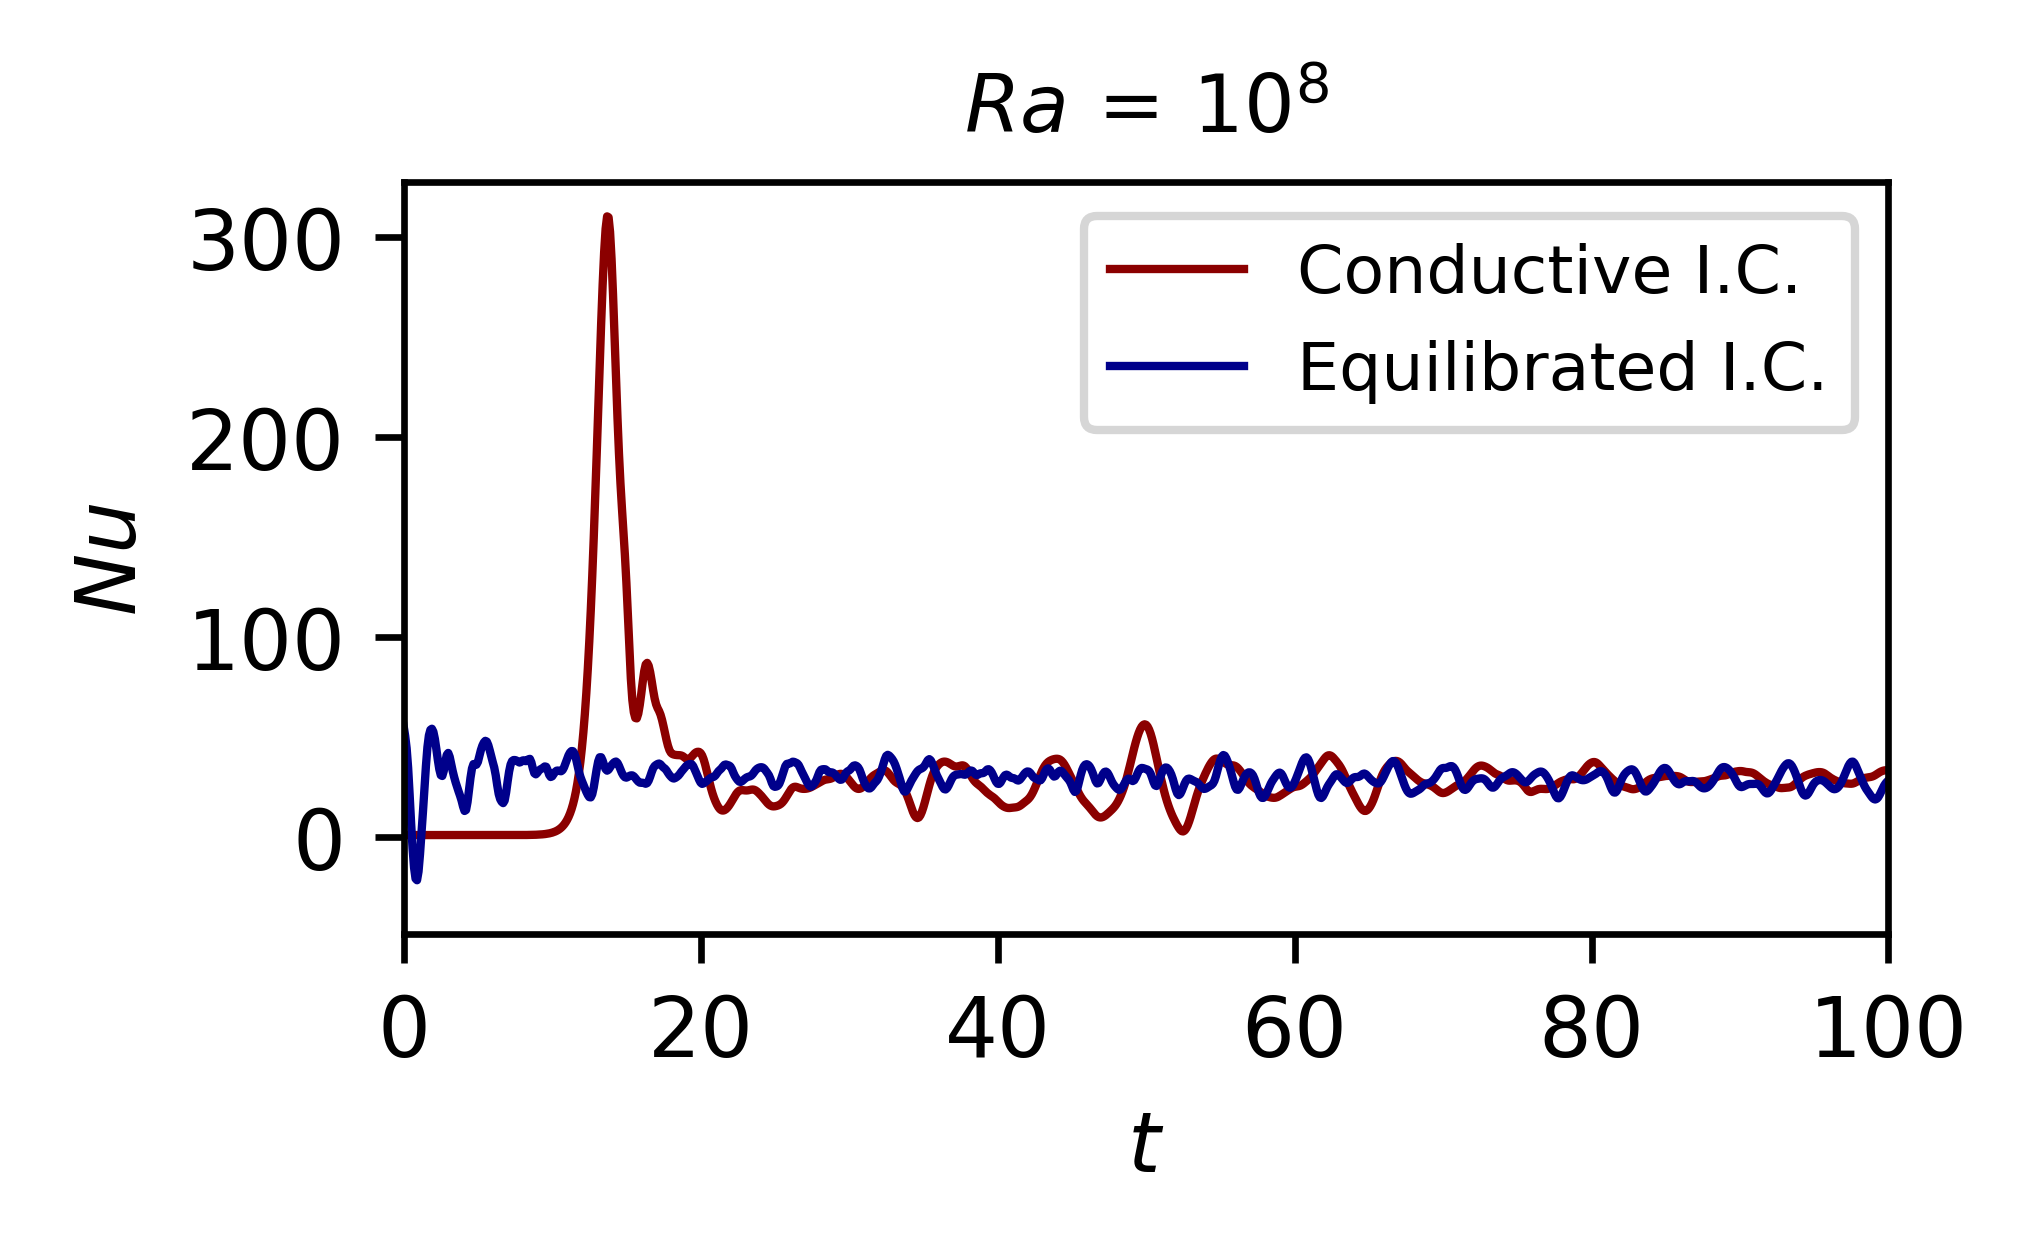
\includegraphics[width=3.4in]{sim_eq_nu.png}
        \caption{Nusselt numbers of simulations performed at $\Ra = 10^8$, initialized with the conductive equilibrium plus thermal noise (black) and the MSTE (blue). 
        MSTE simulations do not undergo a convective-transient period because the characteristic large-scale convective cell structure exists on initialization.}
        \label{fig:nu_sim}
    \end{minipage}
\end{figure}

Simulations initialized with the conductive equilibrium plus low-amplitude thermal noise have a large peak in $\Nu$ early on in their evolution (Figure~\ref{fig:nu_sim}).
This is due to a burst of turbulence which occurs when the convective motions first become nonlinear.
A simulation initialized with the MSTE, however, does not exhibit this transient burst of turbulence, as the large-scale anatomy of convective cells exists on initialization. 
Simulation of this transitional period is prohibitive \cite{Anders_AE}. 
For high $\Ra$ experiments, researchers often ``bootstrap" data by initializing simulations with the results of similar $\Ra$ runs \cite{Verzicco, Johnston}. 
MSTE can be perceived as a set of initial conditions, designed for avoiding the simulation of transitional high Reynolds number flows.

MSTE are laminar, lacking the small-scale structures associated with moderate to high $\Ra$ experiments. 
This is an apparent consequence of the quasilinear assumptions. 
If we perceive MSTE as background states, DNS suggest that plumes, vortex sheets, and other unstable turbulent features inhibit total heat transfer. 
This perspective agrees with conventional models of transitions to turbulent flows, such as Boussinesq's turbulent-viscosity hypothesis \cite{boussinesq_1877}. The emergence of small-scale velocity structures tends to increase total shear \cite{Lecoanet_KH, drazin_reid_2004, pope_2000}, thereby impeding buoyancy-driven flows and decreasing advection in the bulk of the domain. 
We could also attribute the diffuse DNS temperature profile in Figure \ref{fig:T0_profiles} with unsteady boundary-layer penetration and mixing that MSTE do not exhibit.

\begin{figure}
    \begin{minipage}{3.4in}
        \centering
        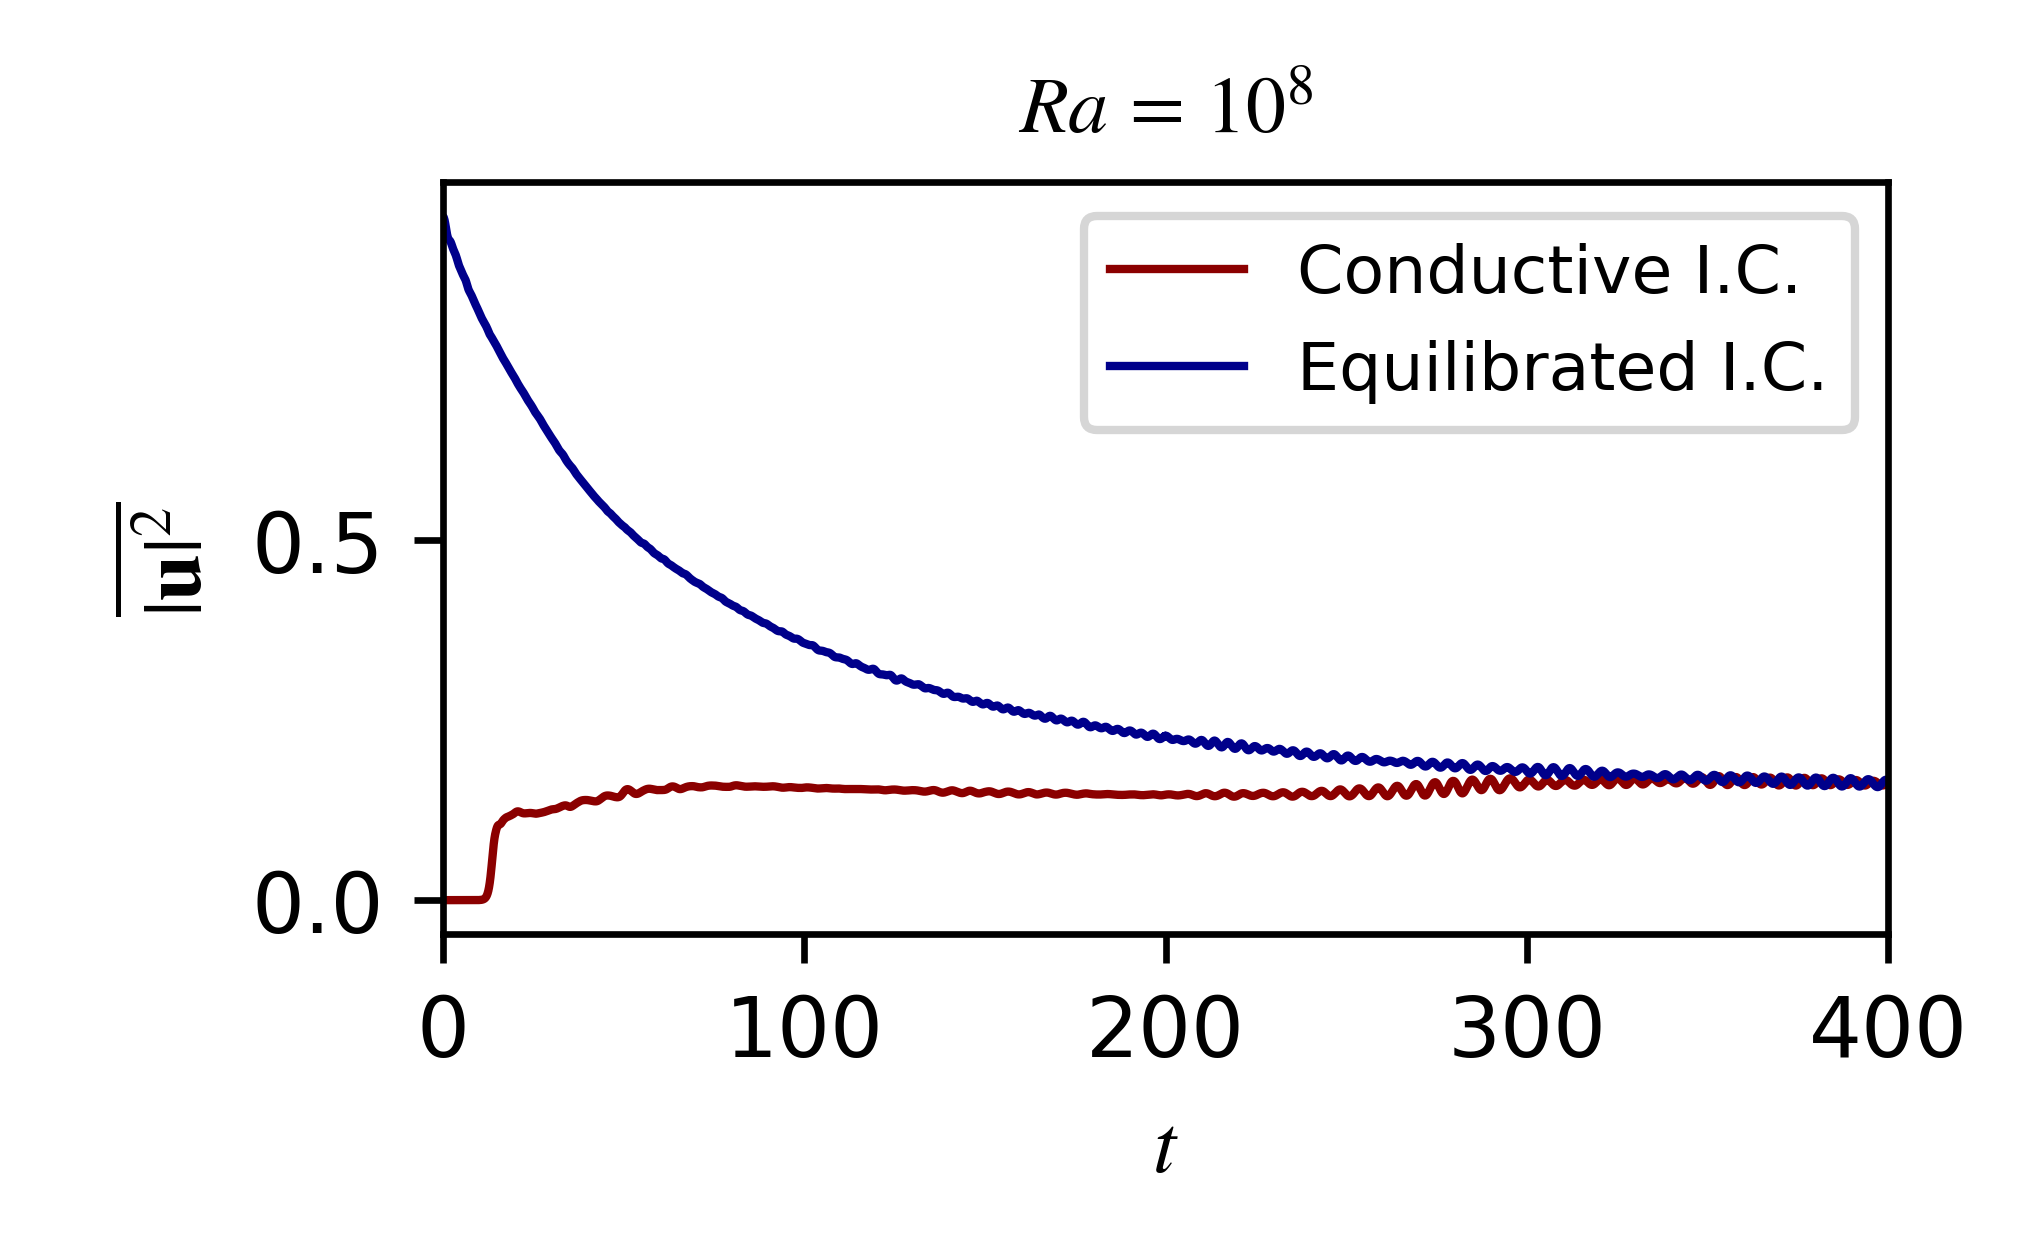
\includegraphics[width=3.4in]{sim_eq_ke.png}
        \caption{Average kinetic energies are reported for the same simulations illustrated in Figure \ref{fig:nu_sim} ($\Ra = 10^8$). 
        The eigenfunctions belonging to MSTE have significantly more kinetic energy than the statistically-steady state. 
        Kinetic equilibrium is achieved on the viscous time-scale $t_{\nu} \sim \sqrt{\Ra / \Pr}$.}
        \label{fig:ke_sim}
    \end{minipage}
\end{figure}

We also find that the average kinetic energies of simulations initialized with MSTE are significantly larger than those found in simulations initialized with the conductive state plus noise, as shown Figure \ref{fig:ke_sim}. 
This is because the MSTE contain strong large-scale flows, which decay on a viscous time-scale
\begin{equation}
    t_{\nu} \sim \sqrt{\frac{\Ra}{\Pr}}. \nonumber
\end{equation}
Consequently, MSTE initial conditions do not reduce the simulation time required to achieve a statistically-steady state---rather they increase it considerably!
This suggests the MSTE background state perspective is partially flawed, as a more useful background state would approximate the kinetic energy with more fidelity.

\section{Discussion}\label{sec:Discussion}
In this paper we describe a new way to study Rayleigh–Bénard convection. 
We compute marginally-stable thermal equilibria (MSTE), which are equilibria of the quasilinear equations.
To compute MSTE, we construct a marginally-stable mean temperature profile and evolved it according to the advective flux of its marginally-stable eigenfunctions, and its own diffusion. 
We assume that at least some modes are always in a marginally-stable configuration. 
The marginal stability constraint then fixes the ratio between advection and diffusion (eigenfunction amplitude $A^2$). 
We use standard root-finding algorithms to solve for the appropriate $A^2$ at each iteration, until, the fixed combination of diffusion and advection sum to a constant flux.
The MSTE calculation is a one-dimensional problem, combining eigenvalue solves, and the time evolution of the one-dimensional mean temperature profile.
Thus, they can be calculated on a single workstation.

The MSTE retain several key features that are prevalent in experiments and simulations: $\Nu \sim\Ra^{1/3}$ scaling, large-scale convective cell structures, and minimum length scale agreement. 
They also exhibit unique and unexpected features: mean temperature gradient-reversals/dips, high kinetic energy flows, and a larger $\Nu$ than other time-invariant solutions. 
When initializing with different mean temperature profiles, we found the same MSTE, suggesting these equilibria might be unique.

Simulations initialized with the MSTE \eq{EQ:mste_ic} do not undergo an early convective transient period, but have faster flows when compared with DNS.
From a dynamical systems perspective, unstable orbits depart from MSTE and approach the global attractor on a viscous time-scale.
This requires more computational effort to achieve relaxation when compared to the conventional conductive initial condition \eq{EQ:linear_ic}.

As previously noted, using the mean temperature in a statistically-steady DNS as a background state for an eigenvalue problem yields positive eigenvalues: the system is in a perpetual state of instability. 
Unstable modes tend to stabilize the system rapidly, creating a negative feedback loop whose average state is linearly unstable. 
We might curtail the disagreement between MSTE and DNS by adjusting our marginal-stability criterion. 
Should the fast and slow time scales not be entirely separate, we might anticipate the long-term persistance of moderately unstable modes. 
To find MSTE, we initialize the time-evolution algorithm with the analytic temperature profile derived by \cite{Shishkina}.
This involves modifying the boundary layer thickness $\delta_0$ to achieve marginal stability.

Instead of imposing marginal stability, we can use quasilinear model to thermally-equilibrate and expand 1D approximations into 2D.
As previously noted, there is no shortage of theories pertaining to the scaling behavior $\Nu \sim \Ra^{\beta}$ \cite{Malkus_1954, Howard_1966, Kraichnan, Spiegel, Castaing, Grossman, Ahlers}.
For large $\Ra$, we can approximate $\delta_0 \approx \Nu^{-1}$ and construct a 1D temperature profile according to \eq{EQ:T0} or some other approximation.
In this way, other 2D quasilinear thermal equilibria can be obtained and analyzed. 

\section*{Acknowledgments}
The authors thank Geoff Vasil, Greg Chini, and Emma Kaufman for their valuable feedback and suggestions. 
We also thank the \texttt{Dedalus} and \texttt{Eigentools} development teams. 
Computations were conducted with support by the NASA High End Computing (HEC) Program through the NASA Advanced Supercomputing (NAS) Division at Ames Research Center on Pleiades with allocation GIDs s2276.

\appendix

\section{Initial buoyancy profile} \label{sec:initial_profile}
We initialize the thermal-equilibration algorithm with \cite{Shishkina}'s analytical thermal boundary layer equation for turbulent Rayleigh-B\'enard convection, given by 
\begin{align}
    \bar{T}_0(\xi) &= \frac{\sqrt{3}}{4\pi} \log \frac{(1 + a\xi)^3}{1 + (a\xi)^3} + \frac{3}{2\pi} \arctan \Big( \frac{4\pi}{9}\xi - \frac{1}{\sqrt{3}} \Big) + \frac{1}{4} \nonumber \\
    \xi &= \frac{z}{\delta_0}, \qquad a = \frac{2\pi}{3\sqrt{3}}\label{EQ:T0}
\end{align}
where $\delta_0$ is the boundary layer height. 
We expect that each $\Ra$ is associated with a unique $\delta_0$ for which $\bar{T}_0(z)$ is marginally-stable. 
It should be noted that when experimenting with various initial profiles $(\tanh, \rm{erf}, \rm{etc.})$, we obtain indistinguishable equilibrated states, implying that solutions may be unique. 
An example of \eq{EQ:T0} is given by the blue curve in Figure \ref{fig:T0_profiles}.

% \begin{multicols}{1}
\section{MSTE Metrics}\label{sec:tables}
\begin{longtable*}{cccccc}
    %\begin{tabular}{cccccc}
    %\hline
    %\begin{longtable}[c]{@{}*{6}{>{\arraybackslash}p{0.15\linewidth}}@{}}
    \quad\quad\quad Ra	\quad\quad\quad	&	\quad\quad\quad		Pr	\quad\quad\quad		&	\quad\quad\quad		$k=2\pi/\Gamma$	\quad\quad\quad		&	\quad\quad\quad		$N_x \times N_z$	\quad\quad\quad		&	\quad\quad\quad		Nu	\quad\quad\quad		&	\quad\quad\quad		Re	\quad\quad\quad\\
    %\hline
    $10^{13/4}$	&	1	&	$\pi$	&	128 $\times$ 65	&	1.056590	&	1.617336\\
    $1.9\times10^3$	&	1	&	$\pi$	&	128 $\times$ 65	&	1.145807	&	2.682155\\
    $2\times10^3$	&	1	&	$\pi$	&	128 $\times$ 65	&	1.212037	&	3.317190\\
    $2.25\times10^3$	&	1	&	$\pi$	&	128 $\times$ 65	&	1.355410	&	4.550975\\
    $2.5\times10^3$	&	1	&	$\pi$	&	128 $\times$ 65	&	1.474455	&	5.537770\\
    $2.75\times10^3$	&	1	&	$\pi$	&	128 $\times$ 65	&	1.575599	&	6.391812\\
    $3\times10^3$	&	1	&	$\pi$	&	128 $\times$ 65	&	1.663162	&	7.159844\\
    $10^{14/4}$	&	1	&	$\pi$	&	128 $\times$ 65	&	1.714193	&	7.624400\\
    $3.5\times10^3$	&	1	&	$\pi$	&	128 $\times$ 65	&	1.808754	&	8.526064\\
    $4\times10^3$	&	1	&	$\pi$	&	128 $\times$ 65	&	1.926775	&	9.740578\\
    $4.5\times10^3$	&	1	&	$\pi$	&	128 $\times$ 65	&	2.025985	&	10.85141\\
    $5\times10^3$	&	1	&	$\pi$	&	128 $\times$ 65	&	2.111714	&	11.88534\\
    $10^{15/4}$	&	1	&	$\pi$	&	128 $\times$ 65	&	2.204811	&	13.09152\\
    $8\times10^3$	&	1	&	$\pi$	&	128 $\times$ 65	&	2.476330	&	17.05494\\
    $10^4$	&	1	&	$\pi$	&	128 $\times$ 65	&	2.648664	&	20.07400\\
    $10^{17/4}$	&	1	&	$\pi$	&	128 $\times$ 65	&	3.122843	&	29.50047\\
    $10^{18/4}$	&	1	&	$\pi$	&	128 $\times$ 65	&	3.665041	&	42.29585\\
    $10^{19/4}$	&	1	&	$\pi$	&	128 $\times$ 65	&	4.287042	&	59.56858\\
    $10^{5}$	&	1	&	$\pi$	&	128 $\times$ 65	&	4.994322	&	82.84462\\
    $10^{21/4}$	&	1	&	$\pi$	&	128 $\times$ 65	&	5.795869	&	114.2355\\
    $10^{22/4}$	&	1	&	$\pi$	&	128 $\times$ 97	&	6.703915	&	156.5252\\
    $10^{23/4}$	&	1	&	$\pi$	&	128 $\times$ 97	&	7.732236	&	213.4031\\
    $10^{6}$	&	1	&	$\pi$	&	128 $\times$ 97	&	8.896615	&	289.7982\\
    $10^{25/4}$	&	1	&	$\pi$	&	256 $\times$ 97	&	10.21546	&	392.2837\\
    $10^{26/4}$	&	1	&	$\pi$	&	256 $\times$ 129	&	11.71065	&	529.6372\\
    $10^{27/4}$	&	1	&	$\pi$	&	256 $\times$ 129	&	13.40898	&	713.6005\\
    $10^{7}$	&	1	&	$\pi$	&	512 $\times$ 129	&	15.34493	&	959.9367\\
    $1.35\times10^{7}$	&	1	&	$\pi$	&	512 $\times$ 129	&	16.46456	&	1119.932\\
    $1.5\times10^{7}$	&	1	&	$\pi$	&	512 $\times$ 129	&	16.87881	&	1182.172\\
    $1.6\times10^{7}$	&	1	&	$\pi$	&	512 $\times$ 193	&	17.13944	&	1222.005\\
    $1.65\times10^{7}$	&	1	&	$\pi$	&	512 $\times$ 193	&	17.26636	&	1241.484\\
    $1.7\times10^{7}$	&	1	&	$\pi$	&	512 $\times$ 193	&	17.39216	&	1260.709\\
    $1.736\times10^{7}$	&	1	&	$\pi$	&	512 $\times$ 193	&	17.48282	&	1274.414\\
    $1.76\times10^{7}$	&	1	&	$\pi$	&	512 $\times$ 193	&	17.54351	&	1283.493\\
    $10^{29/4}$	&	1	&	$\pi$	&	512 $\times$ 193	&	17.58987	&	1290.377\\
    $1.786\times10^{7}$	&	1	&	$\pi$	&	512 $\times$ 193	&	17.60946	&	1293.277\\
    $1.8\times10^{7}$	&	1	&	$\pi$	&	512 $\times$ 193	&	17.64500	&	1298.522\\
    $1.85\times10^{7}$	&	1	&	$\pi$	&	512 $\times$ 193	&	17.77160	&	1317.122\\
    $1.9\times10^{7}$	&	1	&	$\pi$	&	512 $\times$ 193	&	17.89693	&	1335.501\\
    $1.95\times10^{7}$	&	1	&	$\pi$	&	512 $\times$ 193	&	18.02044	&	1353.657\\
    $2\times10^{7}$	&	1	&	$\pi$	&	512 $\times$ 193	&	18.14193	&	1371.593\\
    $2.4\times10^{7}$	&	1	&	$\pi$	&	512 $\times$ 193	&	19.04221	&	1507.890\\
    $2.8\times10^{7}$	&	1	&	$\pi$	&	512 $\times$ 193	&	19.83413	&	1633.418\\
    $10^{30/4}$	&	1	&	$\pi$	&	512 $\times$ 193	&	20.47798	&	1739.647\\
    $4.5\times10^{7}$	&	1	&	$\pi$	&	512 $\times$ 193	&	22.44036	&	2087.182\\
    $10^{31/4}$	&	1	&	$\pi$	&	512 $\times$ 193	&	23.76002	&	2340.822\\
    $10^{8}$	&	1	&	$\pi$	&	768 $\times$ 257	&	27.50669	&	3144.931\\
    $10^{33/4}$	&	1	&	$\pi$	&	768 $\times$ 257	&	31.81154	&	4220.616\\
    $2.15\times10^{8}$	&	1	&	$\pi$	&	768 $\times$ 257	&	33.36657	&	4649.541\\
    $10^{34/4}$	&	1	&	$\pi$	&	768 $\times$ 257	&	36.75427	&	5658.648\\
    $4.64\times10^{8}$	&	1	&	$\pi$	&	896 $\times$ 321	&	40.44652	&	6875.704\\
    $10^{35/4}$	&	1	&	$\pi$	&	896 $\times$ 321	&	42.42917	&	7580.057\\
    $10^{9}$	&	1	&	$\pi$	&	1024 $\times$ 321	&	48.94284	&	10145.79\\
    $10^{37/4}$	&	1	&	$\pi$	&	1024 $\times$ 321	&	56.42926	&	13571.10\\
    $2.15\times10^{9}$	&	1	&	$\pi$	&	1024 $\times$ 321	&	59.13988	&	14935.81\\
    $2.5\times10^{9}$	&	1	&	$\pi$	&	1024 $\times$ 321	&	61.38714	&	16116.94\\
    $10^{38/4}$	&	1	&	$\pi$	&	1024 $\times$ 321	&	65.06338	&	18145.61\\
    $10^{153/16}$	&	1	&	$\pi$	&	1024 $\times$ 321	&	67.42466	&	19511.79\\
    $4\times10^{9}$	&	1	&	$\pi$	&	1024 $\times$ 321	&	68.96487	&	20429.24\\
    $4.64\times10^{9}$	&	1	&	$\pi$	&	1024 $\times$ 321	&	71.58241	&	22019.93\\
    $10^{39/4}$	&	1	&	$\pi$	&	1024 $\times$ 321	&	75.09725	&	24262.22\\
    $10^{10}$	&	1	&	$\pi$	&	1024 $\times$ 321	&	86.68318	&	32430.06\\
    $10^{41/4}$	&	1	&	$\pi$	&	1024 $\times$ 321	&	100.0909	&	43339.02\\
    $2\times10^{10}$	&	1	&	$\pi$	&	1024 $\times$ 321	&	103.0738	&	45995.60\\
    $2.15\times10^{10}$ &	1	&	$\pi$	&	1024 $\times$ 321	&	104.9517	&	47705.08\vspace{0.1in}\\
    %\hline
    %  \end{tabular}
    \caption*{Table S1: Details for numerical solutions with $\Pran=1$ and $\Gamma=2$.  $N_x$ and $N_z$ represent the numbers of Fourier and Chebyshev modes, respectively.}
    {\label{tab:Gamma2}}
    \end{longtable*}
% \end{multicols}


% \bibliographystyle{plain}
\bibliography{he}

\end{document}
